% vim: set wrap

% This template was created May 4th, 2010 by Colin Ophus.  Since my thesis was accepted by the Library of Canada, I believe all of the formatting, page ordering, etc is correct.  To start, fill out all of the definitions below, ie every term after a \def. Then modify the existing chapters and create your own.

% This is a thesis template designed to meet the University of Alberta electronic submission standards.
% It comes with absolutely no guarantees that it will work at all.
% That being said, it should work first try with no need to install additional packages or style files. I designed it with PDFLaTeX in mind, so you should use .png and if you must .jpg and .tiff image files. For the more advanced users, PDF files can be used for any figure or if you change to a DVI intermediary you can use .eps format.

% Known bugs:
% - Unfortunately you will get ~9 warnings for the intro pages.  This is a consequence of removing the numbering from those pages (as required by the U of A faculty of grad studies and research.  I do not know how to correct this.
% - The preface page is double spaced in addition to the abstract page. This is not really a problem, but I would prefer to double space only the abstract.  I have not figured out a good way to do so though.

\documentclass[12pt, letterpaper]{report}

% Define global variables, like names and thesis title
% If you thesis title is more than three lines, you will need to adjust the spacing on the title page.
\def\name{Timo Ewalds}
\def\thesistitle{Playing and Solving Havannah}% using Monte Carlo Tree Search and Proof Number Search}
\def\supervisor{Jonathan Schaeffer}
\def\coma{Ryan Hayward}
\def\comb{Martin Mueller}
\def\comc{Mazi Shirvani}
\def\superloc{Computing Science}
\def\loca{Computing Science}
\def\locb{Computing Science}
\def\locc{Mathematics}
\def\program{Master}  % Your degree
\def\school{University of Alberta}
\def\semester{Fall 2011}  % The convocation period when you submit your thesis:  Spring or Winter, then year
\def\dept{Computing Science}  % Your department

% Add command for degree symbol:   \degree
\newcommand{\degree}{\ensuremath{^\circ}}

% Various packages and appearance changes
% Adjust if desired
\usepackage{amsmath, amssymb, amsthm}
\usepackage{graphicx,color}
\usepackage[left=1.5in, right=1.5in, top=1.5in, bottom=1in, includefoot, headheight=.5in]{geometry}
\parindent 0pt
\parskip 10pt
\renewcommand{\baselinestretch}{1.33}
\numberwithin{equation}{section}
\renewcommand{\bibname}{References}
\renewcommand{\contentsname}{Contents}
\pagenumbering{roman}

\usepackage{havannah}
\renewcommand\HDrawHex{\draw[fill=gray!35]}

\usepackage{fancybox}
\usepackage{tikz}
\usepackage{pgfplots}

\pgfplotsset{
  every axis legend/.append style={
    at={(1.01,1.0)},
    anchor=north west,
    font=\footnotesize,
  },
  width=12cm,
  height=7cm,
}


\usepackage{multirow}

\usepackage{subfig}

%for the euro symbol
\usepackage[gen]{eurosym}

\usepackage{listings}

\lstset{ %
%language=C++,                % choose the language of the code
basicstyle=\footnotesize,       % the size of the fonts that are used for the code
%numbers=left,                   % where to put the line-numbers
%numberstyle=\footnotesize,      % the size of the fonts that are used for the line-numbers
%stepnumber=1,                   % the step between two line-numbers. If it is 1 each line will be numbered
%numbersep=5pt,                  % how far the line-numbers are from the code
%backgroundcolor=\color{white},  % choose the background color. You must add \usepackage{color}
showspaces=false,               % show spaces adding particular underscores
showstringspaces=false,         % underline spaces within strings
%showtabs=false,                 % show tabs within strings adding particular underscores
frame=single,   		% adds a frame around the code
tabsize=3,  		% sets default tabsize to 2 spaces
%captionpos=b,   		% sets the caption-position to bottom
breaklines=true,    	% sets automatic line breaking
breakatwhitespace=false,    % sets if automatic breaks should only happen at whitespace
%escapeinside={\%}{)}          % if you want to add a comment within your code
}



% Bibliography stuff
\usepackage[square, comma, numbers, sort&compress]{natbib}
\renewcommand{\bibsep}{10pt}
\bibliographystyle{unsrtnat}
%\bibliographystyle{ieeetr}

% Customising headers
\usepackage{fancyhdr}
\pagestyle{fancy}
\rhead{}
\lhead{\nouppercase{\textsc{\leftmark}}}
\renewcommand{\headrulewidth}{0pt}
\makeatletter
\renewcommand{\chaptermark}[1]{\markboth{\textsc{\@chapapp}\ \thechapter:\ #1}{}}
\makeatother%

% New chapter headings
\usepackage[grey,utopia]{quotchap}

% PDF hyperlinks
% This is where you change their colouring - feel free to go wild or conservative, it is your thesis after all
\usepackage[colorlinks]{hyperref}
\usepackage[figure,table]{hypcap}
\hypersetup{
  bookmarksnumbered,
  pdfstartview={FitH},
  citecolor={blue},
  linkcolor={blue},
  urlcolor={blue},
  pdfpagemode={UseOutlines}
}
\makeatletter
\newcommand\org@hypertarget{}
\let\org@hypertarget\hypertarget
\renewcommand\hypertarget[2]{%
  \Hy@raisedlink{\org@hypertarget{#1}{}}#2%
}
\makeatother

% Change bulleted lists - feel free to modify this
\renewcommand{\labelitemi}{$\blacktriangleright$}





% Actual text of the thesis starts here
\begin{document}
  \pagenumbering{roman}
  \setcounter{page}{-99}  % So that page numbering won't interfere, -ve numbers don't show
  \thispagestyle{empty}


  % vim: set wrap

  % Titlepage
  \pdfbookmark[0]{Prefatory Pages}{prefatory}
  \pdfbookmark[1]{Title}{title}
%  \vspace{.25in}
%  \title{
  \begin{center}
    \Large{\textbf{\school}}  \\ [.6in]
    \Large{\textbf{\thesistitle}} \\ [.1in]
    \normalsize{by} \\ [.1in]
    \Large{\textbf{\name}}  \\ [.6in]
    \normalsize{A thesis submitted to the Faculty of Graduate Studies and Research \\
    in partial fulfillment of the requirements for the degree of} \\ [0.1in]
    \Large{\textbf{\program}} \\ [.1in]
    \normalsize{\dept} \\ [0.6in]
    \scriptsize{\copyright\:\name} \\
    \scriptsize{\semester} \\
    \scriptsize{Edmonton, Alberta} \\ [0.6in]
    % DO NOT modify this text, it is a requirement
    \scriptsize{Permission is hereby granted to the University of Alberta Libraries to reproduce single copies of this thesis and to lend or sell such copies for private, scholarly or scientific research purposes only. Where the thesis is converted to, or otherwise made available in digital form, the University of Alberta will advise potential users of the thesis of these terms.

The author reserves all other publication and other rights in association with the copyright in the thesis and, except as herein before provided, neither the thesis nor any substantial portion thereof may be printed or otherwise reproduced in any material form whatsoever without the author's prior written permission.}
  \end{center}

  % Examining committee page
  \newpage
  % Begin numbering the pages with Roman numerals
  \pdfbookmark[1]{Examining Committee}{examining}
  \chapter*{Examining Committee}
  \thispagestyle{empty}
     \supervisor, \; \superloc \\ \\
     \coma, \; \loca \\ \\
     \comb, \; \locb \\ \\
     \comc, \; \locc \\ \\
     \comd, \; \locd \\ \\
     \come, \; \loce


  % Dedication
%   \newpage
%  \pdfbookmark[1]{Dedication}{dedication}
%  \chapter*{}
%  \thispagestyle{empty}
%  This thesis is dedicated to\\
%  A person or persons or perhaps some abstract concept.

  % Abstract
  \newpage
  \pdfbookmark[1]{Abstract}{abstract}
  \chapter*{Abstract}
  \thispagestyle{empty}
  \vspace*{-0.7in}
  \renewcommand{\baselinestretch}{1.8}
  \normalsize{

Havannah is a recent game that is interesting from an AI research perspective. Some of its properties, including virtual connections, frames, dead cells and draws are explained. Monte Carlo Tree Search (MCTS) is well suited to play Havannah, but the playing strength can be improved by using heuristic knowledge and a modified rollout policy. A change to the rules in the rollout policy significantly improves play. Combined with several Havannah specific heuristics, a greater than 80\% winning rate, or 300 elo gain, is achieved on all board sizes over an already fairly strong player. This MCTS player is augmented with a few engineering improvements and then used to solve all 6 openings of size 4 Havannah, a game with a state space on the order of $6 \times 10^{15}$ states. Castro, the implementation and test bed, is released open source.

  }

% A second paragraph if you need it
%  \vspace*{-0.2in} \\
%  \normalsize{
%  This is a second abstract paragraph. if you need it.
%  }
  \renewcommand{\baselinestretch}{1.33}

  % Preface
  \newpage
  \pdfbookmark[1]{Preface}{preface}
  \chapter*{Preface}
  \thispagestyle{empty}
  \vspace*{-0.7in}

I've never been very good or interested in playing board games, but I've always had a fascination with how to play them well. I started programming when I was 13 years old, and one of my first projects was to write an AI for tic-tac-toe. This is rather easy, as the game is tiny, but it was a good project for teaching me to program. A few years later I was introduced to mancala, and as a way to understand the game better, I decided to write a program to play it, and in the process, independently reinvented minimax and rediscovered that many games are zero-sum. My mancala program was never any good as I didn't know anything about alpha-beta and wikipedia hadn't been invented yet, but I have always had a greater interest in understanding how the mechanics of the game work than actually playing the game. Writing a strong program is a great challenge, and a very satisfying one if your program becomes a stronger player than you are yourself.

In late 2008 I was introduced to Pentago, an interesting game invented in 2005. It is a 2-player game played on a 6x6 board where each turn is composed of placing a stone and rotating a 3x3 quadrant with the goal of forming 5 in a row. After playing a few rounds and losing badly, I decided to figure out how to write a program to play it so that I could better understand the strategy and tactics. During a few rounds of play I devised a simple heuristic, which on its own is very weak, but when used with alpha-beta is quite strong. With some optimization, my program, Pentagod, became strong enough to easily crush me and my friends.

In early 2010, while taking a computer science course in computer game AI with Martin Mueller, I was tasked with writing a program to play Havannah. Basing my program, Castro, on my earlier work on Pentagod, my program became reasonably strong by program standards, but still quite weak by human standards. In fact, Christian Freeling, the creator of Havannah was so certain that programs would remain weak that he issued a challenge for \euro 1000 to anyone who can beat him in only one in ten games on size 10 by 2012. I continued working on my program after the course finished, implementing techniques mentioned in class or used in other games, trying to use the theoretical properties used in the related game Hex, optimizing my code for pure efficiency and parallelism, and coming up with Havannah specific techniques. In September 2010 I went to Kanazawa Japan to compete in the Computer Games world championship and won 15 out of 16 games, winning the tournament. Soon after I attempted to solve size 4, a small version of the game, and succeeded in January 2011.

This thesis is the story of what it takes to write a strong Havannah player, and how this player was used as the basis of solving size 4 Havannah. Chapter \ref{intro} introduces some of the concepts and motivations for this thesis. Chapter \ref{background} explains the required background knowledge for the algorithms used in the rest of thesis. Chapter \ref{havannah} describes the rules of the game and introduces several properties of the game itself that make writing a program challenging, and a few that can be exploited to increase the playing strength. Chapter \ref{playing} explains how the general techniques were adapted to Havannah and introduces a few Havannah specific heuristics that together lead to a tournament level program. Chapter \ref{solving} explains how the player was used to solve size 4 Havannah and the extra techniques needed to accomplish this goal along with the solution to size 4 Havannah. Chapter \ref{conclusion} provides a summary, and described possible future work.



  % Acknowledgements
  \newpage
  \pdfbookmark[1]{Acknowledgements}{acknowledgements}
   \chapter*{Acknowledgements}
   \thispagestyle{empty}
   \vspace*{-0.7in}
   \small{

I'd especially like to thank Colin Ophus, for playing so many games of Pentago and Havannah with me, and trying to deconstruct the games. His insights and enthusiasm helped me stay motivated and continually improve Castro. Also, I appreciate the thesis template and thesis advice.

Thank you Ryan Hayward, Martin Mueller and Jonathan Schaeffer, for your insights into game playing algorithms, how they apply to other games and possibly to Havannah, and for advising me on my thesis.

Thank you Marcin Ciura for your havannah.sty which made the havannah diagrams easy, and the constant discussion of Havannah ideas.

Thanks to my family and friends, for their constant support as I worked on my masters.

Thank you Christian Freeling, for inventing such an interesting game.

   }




  % Table of contents
  \newpage
  \pdfbookmark[0]{Contents}{contents}
  \pdfbookmark[1]{Table of Contents}{toc}
  \normalsize
  \tableofcontents

  % List of figures
  \newpage
  \pdfbookmark[1]{List of Figures}{listfigs}
  \listoffigures

  % List of tables
  \newpage
  \pdfbookmark[1]{List of Tables}{listtables}
  \listoftables

  % List of symbols
  \newpage
%  \thispagestyle{empty}
%  \pdfbookmark[1]{List of Symbols}{listsymbols}
%  \section*{}
%  \begin{flushright}
%    \huge{List of Symbols}
%  \end{flushright}
%  \vspace{0.4in}
%  \begin{center}
%    \begin{tabular}{rl}
%      Symbol & Meaning\\
%      \hline
%%      $\alpha$      & Upper Bound \\
%%      $\beta$        & Lower Bound \\
%      $pn$           & Proof number \\
%      $dn$           & Disproof number \\
%      $\phi$         & Proof number at an OR node, disproof number at an AND node \\
%      $\delta$       & Disproof number at an OR node, proof number at an AND node \\
%    \end{tabular}
%  \end{center}

  % List of abbreviations
  \newpage
  \thispagestyle{empty}
  \pdfbookmark[1]{List of Abbreviations}{listabbrev}
  \section*{}
  \begin{flushright}
    \huge{List of Abbreviations}
  \end{flushright}
  \vspace{0.4in}
  \begin{center}
    \begin{tabular}{rl}
      Abbreviation & Meaning \\
      \hline
      $\alpha\beta$ & Alpha-Beta algorithm \\
      AI            & Artificial Intelligence \\
      CAS           & Compare And Swap \\
      DAG           & Directed Acyclic Graph \\
%      DFPN          & Depth First Proof Number search \\
      GC            & Garbage Collection \\
      LGR           & Last Good Reply \\
      LGRF          & Last Good Reply with Forgetting \\
      MCTS          & Monte Carlo Tree Search \\
      MPN           & Most Proving Node \\
      PNS           & Proof Number Search \\
      RAVE          & Rapid Action Value Estimate \\
      TT            & Transposition Table \\
      UCB           & Upper Confidence Bounds \\
      UCT           & Upper Confidence bounds as applied to Trees \\
      VC            & Virtual Connection \\

    \end{tabular}
  \end{center}




% ********************************************************************************
  % Main thesis chapters
  % Comment out whatever you are not working on if you want the thesis to build faster
  \newpage
  % Begin numbering the pages with arabic numerals (main thesis body)
  \setcounter{page}{1}
  \pagenumbering{arabic}

  \chapter[Introduction]{\label{intro} \LARGE Introduction and Contributions}
  % vim: set wrap


\section{Introduction}

Artificial intelligence (AI) is an important and exciting field of research with the potential to fundamentally improve the way society functions. One of the earliest and more well-known sub-fields of AI research is games and puzzles. It was once commonly thought that once a computer could play Chess at a world championship level, it would be on par with human intelligence. Deep Blue, the Chess program created by IBM, accomplished world championship level play in 1997, using brute force search. While Chess-playing ability turned out to not be representative of general intelligence, the search techniques pioneered in Chess and similar games are undoubtedly effective at problem solving and are widely applicable to other domains. For AI researchers, the next goal after playing better than humans is to solve the game, in essence to play optimally. Several games, such as Connect 4 and Checkers have been solved, ensuring that a computer player cannot be defeated. Those who aren't working on optimal play are working on harder games than Chess. They are discovering new algorithms and heuristics that  continually push the bounds of what computers can do.

Havannah is a board game invented in 1979 by Christian Freeling. The rules and properties of Havannah are described in detail in Chapter \ref{havannah}. While it is not a popular game, it is interesting from a game research perspective. It is a two player, zero-sum, perfect information game, like Chess, Go and Hex, and like Hex, it is a connection game. Unlike Chess, and like Go, however, it has no known strong heuristic for evaluating a position, making the classical techniques ineffective. Christian Freeling is so confident that computers cannot play Havannah well that in 2002 he placed a \euro 1000 wager that no program could beat him in even one out of ten games on a size 10 board by 2012. This challenge makes it an interesting game for developing newer game playing techniques.

The goal of this thesis is to develop a program that plays strong Havannah on board sizes 4 through 10, and to use this player to solve all 6 openings of the size 4 board.


%- AI is interesting and worthwhile
%- Havannah is representative of AI
%- Optimal play is preferred to merely good/great play

\section{Contributions}

Havannah is closely related to Hex, a similar game that has received significantly more attention over the years. Hex has several mathematical properties that allow a program to ignore certain moves, or to prove the outcome of a game many moves before the end of the game. Several of these properties are shown in Section \ref{sec:properties} to not apply in Havannah, or to apply only in a limited sense. Unlike Hex, draws are possible in Havannah, and detecting these early are key to solving certain positions. A technique for detecting draws once no wins are possible is presented in Section \ref{sec:drawdetect}.

All of the algorithms and ideas presented here were implemented in a program named Castro. Castro is written in C++ and has been released as open source at \url{https://github.com/tewalds/castro}. It includes an MCTS player and several solvers, along with several heuristics. Most of the testing was done using ParamLog, a distributed testing framework written for testing Castro. It has also been released as open source at \url{https://github.com/tewalds/ParamLog}.

With ParamLog, testing a large number of features becomes easy, so all the algorithms and heuristics were tested with multiple values on board sizes 4-10. This is a departure from previous work on Havannah which generally focused only on a single or a few board sizes.

Several knowledge heuristics were tested in Section \ref{sec:knowledge}, including maintaining virtual connections, local reply, locality, edge connectivity, group size and distance to win. Several of these haven't been tested in Havannah before.

Havannah's three winning conditions interact with MCTS in unusual ways, so four novel ring rule variations are introduced and tested in Section \ref{sec:ringrules}.

Testing the many knowledge heuristics and rollout policy features shows that a greater than 80\% winning rate against an already fairly strong baseline can be achieved on all board sizes greater than size 4.

While proof backups have been used in MCTS before, they are shown to be particularly effective in a Havannah player in Section \ref{sec:proofbackups} when combined with a two-ply look-ahead. Chapter \ref{solving} builds on this work and adds threading, draw detection and memory management to solve size 4. The perfect-play solution to size 4 Havannah is presented in Section \ref{sec:size4proof}.

%- Castro, open source Havannah implementation
%  - tested existing heuristics on larger board sizes
%  - distance to win
%  - ring rule variations
%  - strong solver
%- solution to size 4, proof trees



  \chapter[Background]{\label{background} \LARGE Game Playing Techniques}
  

Game playing programs all build a game tree, and then chose the most promising move at the root of the tree.

\section{Minimax}

The minimax algorithm is the foundation of all game playing algorithms and was invented before computers. The goal is the find the minimax value of a state or set of states, or equivalently for a set of moves, and then choose the move with the highest value. All values are from the perspective of the root player. The value of a node for the root player is the maximum of its children nodes, and the minimum for the opponents children. The pseudocode for a simple depth first search version is shown in Figure \ref{fig:minimaxcode}.

\begin{figure}

\begin{lstlisting}
int minimax(State state){
	if(state.terminal())
		return state.value();
	int value;
	if(state.player() == 1){
		value = -INF;
		foreach(state.successors as succ)
			value = max(value, minimax(succ));
	}else{
		value = INF;
		foreach(state.successors as succ)
			value = min(value, minimax(succ));
	}
	return value;
}
\end{lstlisting}

\caption{Minimax Pseudocode}
\label{fig:minimaxcode}

\end{figure}


\subsection{Negamax}

Minimax uses values as taken from a fixed perspective of the root player. This complicates the code with having to minimize for one player and maximize for the other. Noting that $max(a,b) = -min(-a,-b)$, the duplication can be removed by negating the value each time we switch perspective. In this setup all values returned from an evaluation function must be from the perspective of the player who is making the move. The pseudocode for this transformation is shown in Figure \ref{fig:negamaxcode}.

\begin{figure}

\begin{lstlisting}
int negamax(State state){
	if(state.terminal())
		return state.value();
	int value = -INF;
	foreach(state.successors as succ)
		value = max(value, -negamax(succ));
	return value;
}
\end{lstlisting}

\caption{Negamax Pseudocode}
\label{fig:negamaxcode}
\end{figure}

Several algorithms shown later reference the negamax formulation, and mean that the perspective shifts after every move.


\section{Alpha-Beta}\label{sec:alphabeta}

Alpha-beta ($\alpha\beta$) is a refinement of minimax, ignoring or pruning parts of the game tree that are provably unreachable if both players play perfectly. It maintains two bounds to store the minimum value each player is guaranteed given the tree searched so far. When these bounds meet or cross, this is called a cut-off, and the remaining moves don't need to be considered. 

The pseudocode for alpha-beta, written in the negamax formulation is shown in Figure \ref{fig:abcode}. It is a depth first implementation that returns after a maximum depth is reached. If a terminal node is found, the true value is returned, otherwise a heuristic value is returned.

\begin{figure}

\begin{lstlisting}
int alphabeta(State state, int depth, int alpha, int beta){
	if(state.terminal() || depth == 0)
		return state.value();
	foreach(state.successors as succ){
		alpha = max(alpha, -alphabeta(succ, depth-1, -beta, -alpha));
		if(alpha >= beta)
			break;
	}
	return alpha;
}
\end{lstlisting}

\caption{Alpha-beta Pseudocode, shown in the negamax formulation}
\label{fig:abcode}
\end{figure}

The runtime of alpha-beta is highly dependent on the branching factor $b$, search depth $d$, and the number of cut-offs. Minimax has a runtime of $b^d$, as does alpha-beta if it has no cut-offs. Given perfect move ordering, only the first move for the root player will need to be considered, leading to a runtime of $b^{d/2}$, or an exponential speedup. In general, we don't have perfect move ordering, so the runtime will be between these two extremes.

\subsection{Transposition Table}

Transpositions can lead to an exponential blowup in the search space. To minimize the number of transpositions reevaluated, all strong alpha-beta based programs use a transposition table. Transpositions are found by comparing hash values and indexing into a large table. Sometimes a hash table is used, but usually the number of nodes searched is too big to store in memory, so a simple replacement policy is used. The simplest is to use the hash value as an index into a large array of values, replacing the previous node that indexed to the same location.

In many games this leads to a large speedup as the number of nodes searched is decreased dramatically.


\subsection{Iterative Deepening}

The runtime of alpha-beta is exponential in the search depth, and the strength of a player is dependent on a large search depth. If the algorithm is stopped before completion, the best move may not have been explored at all, so a shallower search that finishes is likely better than a deeper search that doesn't. Thus we start with a shallow search, and run a deeper search if we have time. This is not a big waste of work since the majority of the runtime is spent at the deepest level anyway. Iterative deepening allows alpha-beta to act as a breadth-first search with the memory overhead of a depth-first search.

Iterative deepening, when combined with a transposition table, also gives better move ordering. A nodes value from the previous iteration is going to be a more accurate estimate of the value of a node than a heuristic estimate without a search. As we saw in section \ref{sec:alphabeta}, better move ordering can lead to an exponential speedup, easily offsetting the overhead from searching the shallow depths multiple times.

\subsection{History Heuristic}

A good move ordering can lead to many cutoffs and the associated speed increase. The history heuristic is a game independent move ordering heuristic that works by giving higher priority to moves that lead to cutoffs elsewhere in the tree. If a particular move gives a cutoff, it's quite likely that it will also give a cutoff for all of its siblings and so should have a higher priority there. This does assume that similar moves in different part of the tree are related.

\subsection{Other extensions}

Negascout, killer move, quiescence search, etc. Are these worth including at all?





\section{Proof Number Search} \label{sec:PNS}

pseudocode?

Proof Number Search (PNS) is a best-first search used to answer binary questions such as the outcome of a 2-player game starting from a given state. Being a binary outcome with the minimax property, it is well represented as an AND/OR tree when all values are from the perspective of the root player. Each node in the tree can have one of three values: Proven/Win, Disproven/Loss, or Unknown. All nodes store 2 numbers that show how close it is to be proven or disproven. The proof number (pn) is the minimum number of leaf nodes in the subtree that must be proven for the node to be proven. The disproof number (dn) is the minimum number of leaf nodes in the subtree that must be disproven for the node to be disproven. Some leaf nodes, if solved, will change the proof number of the root. Other leaf nodes, if solved, will change the disproof number of the root. Others, if solved, won't affect the proof or disproof numbers of the root. The Most Proving Nodes (MPN) are the intersection of the set that affect the proof number and the set that affect the disproof number at the root. Solving a Most Proving Node will definitely affect either the proof or disproof number of the root. Every tree is guaranteed to have at least one most proving node. Proof Number search grows its tree by continually expanding a most proving node. Proof Number search can be split into 3 phases: descent, expansion, and update.

The most proving node is found during the descent phase. It can be found by selecting the child with the minimum proof number when at an OR node and by selecting the child with the minimum disproof number when at an AND node, applying this iteratively until a leaf node is reached. This leaf node is an MPN.

Once the most proving node $n$ is found, it is expanded, initializing all non-terminal children with $n_i.pn = 1, n_i.dn = 1$, winning children with $n_i.pn = 0, n_i.dn = \infty$ and losing children with $n_i.pn = \infty, n_i.dn = 0 $, where $n_i$ refers to the $i^{th}$ child of $n$.

After expansion, the proof and disproof numbers of all the ancestors of the most proving node must be updated using these formulas. For OR nodes: $$ n.pn = \displaystyle\min\limits_{i=0}^k n_i.pn,\quad n.dn = \displaystyle\sum\limits_{i=0}^k n_i.dn $$ For AND nodes: $$ n.pn = \displaystyle\sum\limits_{i=0}^k n_i.pn, \quad n.dn = \displaystyle\min\limits_{i=0}^k n_i.dn $$ Note how this backs up a single win at an OR node as a win, or a single loss at an AND node as a loss. It also backs up all losses at an OR node as a loss, or all wins at an AND node as a win. % Everywhere else it represents the optimistic lower bound on the number of nodes that must be (dis)proven to (dis)prove the current node.

These three phases are repeated until the root is solved or the tree grows too big to be stored in memory. At the root, if $r.pn = 0$ it is solved as a win, or if $r.dn = 0$ it is solved as a loss, otherwise it is still unknown.

\begin{figure}
\centering
\ovalbox{
\begin{tikzpicture}[
	level distance=15mm,
	level 1/.style={sibling distance=60mm},
	level 2/.style={sibling distance=35mm},
	level 3/.style={sibling distance=15mm},
	]
\node [rectangle,draw] (z){$a \frac{1}{2}$}
  child {node [circle,draw] {$b \frac{1}{2}$}
    child {node [rectangle,draw] {$d \frac{0}{\infty}$}
      child {node [circle,draw,label=below:?] {$h \frac{1}{1}$}}
      child {node [circle,draw,label=below:win] {$i \frac{0}{\infty}$}}
    }
    child {node [rectangle,draw] {$e \frac{1}{2}$}
      child {node [circle,draw,label=below:?] {$j \frac{1}{1}$}}
      child {node [circle,draw,label=below:loss] {$k \frac{\infty}{0}$}}
      child {node [circle,draw,label=below:?] {$l \frac{1}{1}$}}
    }
  }
  child {node [circle,draw] {$c \frac{\infty}{0}$}
    child {node [rectangle,draw,label=below:loss] {$f \frac{\infty}{0}$}}
    child {node [rectangle,draw,label=below:?] {$g \frac{1}{1}$}}
  };
\end{tikzpicture}}
\caption{Proof Number search tree, Squares are OR nodes, Circles are AND nodes, proof numbers are on top, disproof numbers on the bottom, based on \cite{winands2003-PDS-PN}}
\label{fig:pntree}
\end{figure}

Consider the tree in Figure \ref{fig:pntree}. The most proving node is found by following the edges $a \rightarrow b \rightarrow e \rightarrow j$. If $j$ has a child that is a win, it would be backed up as a win at $j$, leading to a win at $e$, and a win at $b$, giving the root player a winning move from the root. With $a.pn = 1$ at the root, only 1 node was needed to be proven as a win for the root to also be proven as a win. If both $j$ and $l$ were proven to be losses, then $e$ would be a loss, leading $b$ to also be a loss, and consequently the root to also be a loss. This is reflected in $a.dn = 2$ at the root. If, however, $j$ has 1 non-terminal child $m$ and no terminal children, $m$ would have $m.pn = 1, m.dn = 1$ and would be the new MPN. If $j$ has 2 non-terminal children and no terminal children, $j.pn = 2, j.dn = 1$, and $l$ would be the new MPN. 

This algorithm selects nodes based on the shape and value of the tree, using no domain or game specific heuristic. It is guided towards slim parts of the tree, areas where there are few moves available, or where many moves are forced. In many games it is advantageous to have more moves available, or higher mobility, than your opponent. Proof Number search is very fast at solving these positions. In games or positions where the branching factor is constant or consistent, with few forced moves, Proof Number search approximates a slow breadth-first search, and thus isn't very fast.

Being a best-first search algorithm, the whole tree must be kept in memory, since any node could become the MPN and therefore be searched at any time. This makes it a very memory intensive search algorithm, with many of the variants attempting to reduce memory usage, allowing bigger problems to be solved.

One simple optimization is to stop the update phase once the proof and disproof numbers don't change. This often happens when siblings have the same value, causing the sibling to be the new MPN. A new search can be started from this node instead of from the root. A simple memory optimization is to remove and reuse the memory of subtrees under a proven or disproven node.

\subsection{The Negamax Formulation} \label{sec:NegaPDS}

\begin{figure}
\centering
\ovalbox{
\begin{tikzpicture}[
	level distance=15mm,
	level 1/.style={sibling distance=60mm},
	level 2/.style={sibling distance=35mm},
	level 3/.style={sibling distance=15mm},
	]
\node [rectangle,draw] (z){$a \frac{1}{2}$}
  child {node [rectangle,draw] {$b \frac{2}{1}$}
    child {node [rectangle,draw] {$d \frac{0}{\infty}$}
      child {node [rectangle,draw,label=below:?] {$h \frac{1}{1}$}}
      child {node [rectangle,draw,label=below:loss] {$i \frac{\infty}{0}$}}
    }
    child {node [rectangle,draw] {$e \frac{1}{2}$}
      child {node [rectangle,draw,label=below:?] {$j \frac{1}{1}$}}
      child {node [rectangle,draw,label=below:win] {$k \frac{0}{\infty}$}}
      child {node [rectangle,draw,label=below:?] {$l \frac{1}{1}$}}
    }
  }
  child {node [rectangle,draw] {$c \frac{0}{\infty}$}
    child {node [rectangle,draw,label=below:loss] {$f \frac{\infty}{0}$}}
    child {node [rectangle,draw,label=below:?] {$g \frac{1}{1}$}}
  };
\end{tikzpicture}}
\caption{Proof Number search tree using the Negamax formulation, all nodes are OR nodes, $\phi$ is on top, $\delta$ is below, based on \cite{winands2003-PDS-PN}}
\label{fig:negamaxtree}
\end{figure}

Just like minimax can be written in the negamax formulation, so too can proof number search. The Proof number at an OR node is the same as the Disproof number at an AND node, and is named $\phi$ (phi). Similarly, the Proof number at an AND node is the same as the Disproof number at an OR node, and is named $\delta$ (delta). Instead of considering all nodes to be from the one player's perspective, all nodes are considered to be from the player who is making the move at that node. This shift in perspective greatly simplifies the code for all variants of proof number search.

Figure \ref{fig:negamaxtree} shows the same tree as in Figure \ref{fig:pntree}, except using the negamax formulation. Note how all nodes are now OR nodes, and the proof and disproof numbers are exchanged in the nodes that were previously AND nodes.

Given this shift in perspective, the descent and update formulas need to be corrected. The new descent move selection is always to choose the child with the minimum delta. The new update formulas are: $$ n.\phi = \displaystyle\min\limits_{i=0}^k n_i.\delta, \quad n.\delta = \displaystyle\sum\limits_{i=0}^k n_i.\phi $$

\begin{figure}

\begin{lstlisting}
int pns(State state){
	Node root = initnode(state);
	while(root.phi != 0 && root.delta != 0) search(root, state);
	return (root.phi == 0 ? PROVEN : DISPROVEN);
}
void search(Node node, State state){
	if(node.numchildren == 0){ //found MPN
		foreach(state.successors as succ)
			node.addchild(initnode(succ));
	}else{
		do{
			Node child = node.child_min_delta();
			search(child, state.move(child.move));
			bool changed = updatePD(node);
		}while(!changed && node.phi != 0 && node.delta != 0);
	}
}
Node initnode(State state){
	Node node; node.move = state.lastmove();
	if(state.win()){       node.phi = 0;   node.delta = INF; }
	else if(state.loss()){ node.phi = INF; node.delta = 0;   }
	else{                  node.phi = 1;   node.delta = 1;   }
	return node;
}
bool updatePD(node){
	int phi = INF, delta = 0;
	foreach(node.children as child){
		phi = min(phi, child.delta);
		delta = delta + child.phi;
	}
	bool changed = (node.phi == phi && node.delta == delta);
	node.phi = phi; node.delta = delta;
	return changed;
}
\end{lstlisting}

\caption{Proof Number Search Pseudocode, shown in the negamax formulation, with the optimization to not propagate up if no changes occur}
\label{fig:pnscode}
\end{figure}

The pseudocode for Proof Number Search in the negamax formulation is shown in Figure \ref{fig:pnscode}.


\subsection{Transposition Table}

Proof number search uses an explicit tree which must be kept in memory, but the tree required is often bigger than available memory. One common approach to bounding the memory needed is to store the nodes in a transposition table instead of an explicit tree. This has the benefit of bounded memory as well as saving computation and memory on transpositions, at the cost of having to recompute nodes that are replaced in the transposition table. Even when a node needs to be recomputed, its children are often still in the transposition table, allowing for a quick recomputation. In many cases the transposition table can be several orders of magnitude smaller than would be needed to store the explicit tree.


\subsection{DF-PN: Depth First Proof Number search} \label{sec:DF-PN}

Depth First Proof Number search (DF-PN)\cite{nagai1999-DFPN} uses two thresholds which are set to express how long the MPN stays in the current subtree. The thresholds are calculated based on the realization that there is no need to update the parents $\phi$ and $\delta$ and do a new move selection if the next descent will go to the same child node. As long as the child's $\delta$ is smaller or equal to all of its siblings, an MPN still lies in its subtree. By staying within this subtree, fewer updates are needed, and locality is maintained, using fewer active nodes and needing less recomputation.

$n.th_\phi$ and $n.th_\delta$ are both set to $\infty$ at the root. $n.th_\phi$ and $n.th_\delta$ are computed as follows: $$n_c.th_\phi = n.th_\delta + n_c.\phi - \displaystyle\sum\limits_{i=0}^k n_i. \phi$$ $$n_c.th_\delta = min(n.th_\phi, n_2.\delta + 1)$$ where $n_c$ refers to the child with the smallest $\delta$ and $n_2$ is the child with the second smallest $\delta$. The search process continues at each node until $n.\phi \geq n.th_\phi$ or $n.\delta \geq n.th_\delta$.


\subsection{DF-PN+: DF-PN with Heuristics} \label{sec:DF-PN+}

So far proof number search assumes that all leaf nodes are equally hard to prove, using only proof and disproof numbers, or more generally, the shape of the tree. DF-PN+ adds two types of heuristic evaluation \cite{nagai-thesis}. 

$h(n)$ is a heuristic evaluation of the expected difficulty of proving or disproving a node and its subtree. DF-PN has a constant $h(n) = 1$. A small value means that this node is expected to be easy to (dis)prove while a big value means this node is expected to be hard to (dis)prove. This value is used at node initialization of non-terminal nodes: $$n.\phi = h_\phi(n), \quad n.\delta = h_\delta(n)$$

$cost(n, n_c)$ is a cost for moving from a node to a child, and affects the shape of the tree. DF-PN has a constant $cost(n, n_c) = 0$. Small values encourage narrow and deep trees while large values encourage wide and shallow trees. This value is a penalty to going deeper, and could be used to encourage deeper trees on moves that are evaluated to be better, or to find shallower solutions.

Adding a non-zero $cost$ function means changing the update formulas: $$ n.\phi = \displaystyle\min\limits_{i=0}^k (n_i.\delta + cost_\delta(n, n_c))$$ $$n.\delta = \displaystyle\sum\limits_{i=0}^k (n_i.\phi + cost_\phi(n, n_c))$$ as well as the threshold formulas:
$$n_c.th_\phi = n.th_\delta + n_c.\phi - \displaystyle\sum\limits_{i=0}^k (n_i.\phi - cost_\delta(n, n_i))$$ $$n_c.th_\delta = min(n.th_\phi, n_2.\delta + cost_\phi(n, n_2) + 1) - cost_\phi(n, n_c)$$

While the values initialized by $h$ are overwritten when its children are expanded, the $cost$ persists until the node is solved. Given fast and effective $h$ and $cost$ functions, DF-PN+ can solve problems significantly faster than DF-PN.

\subsection{The $1+\epsilon$ Trick} \label{sec:epstrick}

One weakness of Proof Number search in general is it requires a large amount of memory to store the tree. Depth first variants and transposition tables help, but many problems we want to solve need trees that are several orders of magnitude bigger than available memory. In cases where the memory limit is particularly tight, DF-PN can spend a huge amount of time regenerating subtrees. To reduce this effect, the $1+\epsilon$ Trick \cite{pawlewicz2007epsilon} increases the thresholds exponentially instead of linearly.

Consider the case where two children of the root (so $\infty$ thresholds) are both promising, but also hard to solve. Since Proof Number search likes keeping all children at similar values, the two will get roughly equal time. Once the subtrees become big, the time spent on one will overwrite the nodes from the other tree. Once its $\delta$ exceeds the other, the search will switch, taking up a large amount of memory, and overwriting the nodes from the subtree of the first child. Since the threshold is one higher than the second smallest, they will swap every time the tree gets rebuilt to exceed the other child by one. This linear increase in the threshold can mean an exponential increase in time.

If the threshold was not simply the second smallest + 1, but instead a multiple of it, the investment into this subtree wouldn't be overwritten so easily by its equally challenging siblings. The $1 + \epsilon$ trick therefore is to replace the $n_c.th_\delta$ threshold from DF-PN with $$n_c.th_\delta = min(n.th_\phi, n_2.\delta*(1 + \epsilon))$$ where $\epsilon$ is some small positive value. This way $n_c.th_\delta$ increases by a constant multiple instead of a constant. It leads to $n_c$ being called at most $log_{1+\epsilon}n.th = O(log n.th)$ times instead of linear times before reaching its parent's threshold.

This trick encourages DF-PN to be even more depth-first, causing lower memory usage, more efficient usage of the transposition table, and reducing the number of node recalculations. Note that it no longer follows the same order as the original PNS, sometimes expanding a node that isn't an MPN, and therefore it may do an unbounded amount of extra work.

$\epsilon = 0.25$ has been shown to work well in practice.


\section{Monte Carlo Tree Search}

For games where a very fast and strong evaluation function exists, alpha-beta is likely to be fast and strong, but no good heuristic is known for many games including Go and Havannah. Monte Carlo Tree Search (MCTS) is an algorithm for building and exploring a game tree that is based on statistics instead of a heuristic evaluation function. MCTS avoids using a heuristic by building its tree as guided by playing random games. While the random games have a very low playing strength, in aggregate random games will favour the player that is in a better position.

MCTS consists of four phases which together are called a simulation. Each simulation adds some experience to the tree, updating the expected chance of winning for the nodes it traverses. These winning rates are stored as the number of wins and the number of simulations through a node. The notation is: $n.v$ for the winning rate and $n.n$ for number of simulations. The four phases are:
\begin{description}
\item[Descent] This phase descends the game tree from the root to a leaf node N in the game tree. At each node one of the available moves is selected according to some criteria based on the current winning rate and possibly heuristic knowledge. When the Upper Confidence Bounds (UCB) formula is used, this is called Upper Confidence Bounds applied to Trees (UCT), but other formulas such as RAVE have been developed and are commonly used.
\item[Expansion] If the node N has experience from a previous simulation, its children are expanded, increasing the size of the tree.
\item[Rollout] A random game is played from N through the newly expanded children, to the end of the game. Heuristics can be used to make the moves less random and more representative of a real game. The strength of the overall algorithm is highly dependent on the average outcome of the random games being representative of the strength of the position.
\item[Back-propagation] The outcome of the random game in the rollout is back propagated to the moves chosen in the tree. The winning rate of the moves made by the player that won the rollout is increased while winning rate of the moves by the player that lost the rollout is decreased.
\end{description}

...diagram needed...

These four steps are repeated continually until a stopping condition is reached, such as running out of time or memory. At this point a move is chosen by some criteria. The three most common criteria are: most simulations, most wins, and highest lower confidence bound on winning rate. The most simulations is the most conservative, but if a counter-move was found late in the game, it may still be the most simulated even if it doesn't have the highest winning rate. The most wins is a little less conservative and will favour a late new-comer if it has almost caught up. The highest winning rate is quite risky since it may favour a move that has a very small subtree where a good counter move exists but hasn't been found yet. To deal with that a lower bound can be used, but a large confidence interval should be used to avoid choosing risky moves.

The pseudocode for MCTS is shown in Figure \ref{fig:mctscode}.

\begin{figure}

\begin{lstlisting}
Move mcts(State state){
	Node root = Node(state);
	while(!timeout)
		search(root, state);
	return root.bestchild();
}
int search(Node node, State state){ //0 = loss, 1 = win
	//rollout
	if(node.numchildren == 0 && node.sims == 0){
		while(!state.terminal())
			state.randmove();
		return (state.win() ? 1 : 0);
	}

	//expand
	if(node.numchildren == 0)
		foreach(state.successors as succ)
			node.addchild(Node(succ));

	//descent
	Node best;
	foreach(node.children as child)
		if(best.value() < child.value())
			best = child;

	int outcome = 1 - search(best, state.move(best.move));

	//back-propagate
	best.sims += 1;
	best.wins += outcome;
	return outcome;
}
\end{lstlisting}

\caption{Monte Carlo Tree Search Pseudocode, shown in the negamax formulation}
\label{fig:mctscode}
\end{figure}


Many extensions have been developed to increase the playing strength of MCTS. Some of these are explained below.

\subsection{UCT: Upper Confidence bounds as applied to Trees}

The most common and most famous formula in MCTS is UCT. It derives from Upper Confidence Bounds (UCB), which is famously used on the multi-armed bandit problem. It is used to balance exploitation and exploration when multiple options are available and each option returns a random distribution of reward. The amount of regret, ie the number of plays to non-optimal arms, should be minimized to maximize reward in the long term.

The UCT formula is: $$n_i.v + c*\sqrt{\frac{ln(n.n)}{n_i.n}}$$ where $c$ is a tunable constant to balance the exploration rate. This formula is used in the descent phase of MCTS to chose which move to make. Intuitively, moves with high winning rate should be exploited more, but moves with a small number of simulations as compared to the parent should be explored to improve the confidence. This formula is guaranteed to converge on the optimal move given infinite time and memory.




\subsection{RAVE: Rapid Action Value Estimate}

In basic MCTS many simulations are run per second, but the information about which moves were made during the rollouts is unused. A win or a loss is composed of many moves which contributed to that outcome, and often good moves during a rollout are also good moves if made earlier during the rollout or during the descent phase. This is a similar realization that lead to the History Heuristic. Thus, we can keep a winning rate for each move during the rollouts and use this to encourage exploration of moves that do well during rollouts. This information is gathered much quicker than pure experience, though it is less correlated to success, so should be phased out as real experience is gained. The notation used is $n.r$ for the rave winning rate and $n.m$ for the number of rave updates for a node.

Usually rave experience and real experience are combined as a linear combination, starting as only rave experience and asymptotically approaching only real experience:
$$ \beta*n_i.v + (1-\beta)*n_i.r $$
Several formulas for $\beta$ have been proposed. The simplest two formulas for $\beta$ are $$\beta = \frac{k}{k+n_i.n}$$ $$\beta = \sqrt{\frac{k}{k+3*n_i.n}}$$ both of which have a tunable constant $k$ which represents the midpoint, so how many simulations are needed for the rave experience and real experience to have equal weight.

David Silver computed an optimal formula for $\beta$ under the assumption of independence of estimates:
$$\beta = \frac{n_i.r}{n_i.n+n_i.r+4*n_i.n*n_i.r*b^2}$$
where $b$ is a tunable rave bias value.

In practice, RAVE leads to a large increase in playing strength for games such as Go and Havannah where the assumption that a good move is also good if played earlier.

\subsection{Heuristic Knowledge}\label{sec:heuristicknowledge}

While UCT is guaranteed to converge given infinite time, game specific knowledge can encourage it to find good moves faster. When a node is expanded, its children all start with no experience, so the default policy is to chose between them randomly. The simulation is going to be more representative of a good game, and lead to a better understanding of the minimax value if it chooses a good move first. Eventually the best move will receive the majority of the simulations, and we'll do better if this is true right from the beginning. Each game has its own heuristics, and Havannah specific ones are described in later chapters, but the way these heuristics is used is game independent.

The first way heuristic knowledge is used is to simply add fake experience to a node. Instead of initializing a node as $n_i.v = 0, n_i.n = 0$, good moves can be initialized with $n_i.v = c, n_i.v = c$, where c is a tunable constant, which effectively means that this node has some amount of wins attributed to it before any simulations have gone through it. This has the effect of allowing the node to look good for the first while even if it is unlucky, but the extra simulations will fade over time as the few extra wins becomes insignificant in the long run. Bad moves can similarly be initialized with fewer wins than simulations effectively depressing its early winning rate. Depending on your implementation, this may encourage the first few simulations to avoid the good moves though, due to their smaller confidence bounds compared to similar moves with the same high winning rate, which has the effect of making the grandparent move look bad. This knowledge could also be added as fake rave experience as well as or instead of to normal experience.

The other way heuristic knowledge is used is to add a knowledge term to the value formula. This leaves the the experience and confidence bounds alone, but gives a boost for the first few simulations to nodes with higher knowledge. This has the added benefit of being able to order the nodes by how large of a boost is given. The knowledge term should fall off with increasing experience. Two suggested knowledge terms are: $$\frac{n_i.k}{log(n_i.n)}, \quad \frac{n_i.k}{\sqrt{n_i.n}}$$ where $n_i.k$ is the knowledge value for the node $n_i$.


\subsection{Rollout Policy}

As mentioned above, the strength of MCTS is highly dependent on the average outcome of the rollouts being representative of the strength of the position. When a player who is in a good position has an easy defence to a devastating attack, but fails to defend, the outcome is not representative of the strength of the original position. Decreasing the randomness by enforcing defences against devastating attacks can bias the outcome, but usually leads to higher quality and more representative games, leading to a stronger player. Most rollout policies used in real programs are game specific, but a few game independent ones are mentioned here.

Instead of pure random, a weighted random scheme can be used. Moves that have good experience in the tree can be selected at a higher probability to poor moves. This could be based on real experience, rave experience or heuristic knowledge as described in the section \ref{sec:heuristicknowledge}.

The Last Good Reply scheme can be used, where the moves made by the player that won a rollout are saved for use in later rollouts when similar situations occur. When these moves fail to lead to a win in a later rollout, they may be removed from the list of replies.

All possible moves can be checked to see if they lead to an instant win, in which case that move should be made. Similarly if this turn is skipped would each move lead to an instant loss if not made, in which case the defensive should be forced.



\subsection{Other extensions}

should any of these be described?

\begin{itemize}
\item parallelization
\item dynamic widening
\item Solution backups
\item multiple rollouts per simulation
\item avoid symmetries or transpositions
\item first player urgency
\end{itemize}














  \chapter[Havannah]{\label{havannah} \LARGE Rules and Properties of Havannah}
  %%
%% This is file `havannah.sty',
%% generated with the docstrip utility.
%%
%% The original source files were:
%%
%% havannah.dtx  (with options: `package')
%% 
%% LaTeX package for Havannah diagrams
%% 
%% Copyright (C) 2010 Marcin Ciura
%% 
\NeedsTeXFormat{LaTeX2e}
\ProvidesPackage{havannah}[2010/06/06 LaTeX havannah package]
\RequirePackage{tikz}
\newcommand\HLetterCoordinates{%
  a,b,c,d,e,f,g,h,i,j,k,l,m,n,o,p,q,r,s,t,u,v,w,x,y,z}
\newcommand\HCoordinateStyle[1]{\sffamily#1}
\newcommand\HMoveNumberStyle[1]{\sffamily#1}
\newcommand\HDrawHex{\shadedraw[
  shading=radial,inner color=gray!30,outer color=gray!70]}
\newcommand\HWhiteStone{\node[
  circle,draw=black,inner sep=0.6pt,fill=white,
  minimum size=\HStoneDiameter]}
\newcommand\HBlackStone{\node[
  circle,draw=black,inner sep=0.6pt,fill=black,text=white,
  minimum size=\HStoneDiameter]}
\newcommand\HTransparentStone{\node[
  circle,draw=black,inner sep=0.6pt,
  minimum size=\HStoneDiameter]}
\newcommand\HBeforeOddMove{}
\newcommand\HBeforeEvenMove{}
\newcommand\HBeforeStone{}
\newcommand{\h@draw@hex}[1]{%
  \HDrawHex (#1)
    ++(-2\h@one@third@hex@wd,0)--
    ++(\h@one@third@hex@wd,-\h@half@hex@ht)--
    ++(2\h@one@third@hex@wd,0)--
    ++(\h@one@third@hex@wd,\h@half@hex@ht)--
    ++(-\h@one@third@hex@wd,\h@half@hex@ht)--
    ++(-2\h@one@third@hex@wd,0)--
    cycle;
}
\newif\ifh@numbered@moves
\newif\ifh@show@coordinates
\newif\ifh@show@hexes
\pgfkeys{%
  /h@havannah@board/.cd,
  board size/.store in=\h@board@size,
  coordinate style/.is choice,
  coordinate style/classical/.code={%
    \def\h@draw@board{\h@draw@classical@board}},
  coordinate style/little golem/.code={%
    \def\h@draw@board{\h@draw@little@golem@board}},
  hex height/.store in=\h@hex@height,
  show coordinates/.is if=h@show@coordinates,
  show hexes/.is if=h@show@hexes,
  board size=10,
  coordinate style=little golem,
  hex height=17.5pt,
  show coordinates=true,
  show hexes=true,
  /h@hex@board/.cd,
  top left color/.is choice,
  top left color/white/.code={%
    \def\h@top@left@color{\HWhiteStone}%
    \def\h@bottom@left@color{\HBlackStone}%
  },
  top left color/black/.code={%
    \def\h@top@left@color{\HBlackStone}%
    \def\h@bottom@left@color{\HWhiteStone}%
  },
  board size/.store in=\h@board@size,
  hex height/.store in=\h@hex@height,
  relative stone size/.store in=\h@relative@stone@size,
  show coordinates/.is if=h@show@coordinates,
  show hexes/.is if=h@show@hexes,
  top left color=black,
  board size=11,
  hex height=17.5pt,
  relative stone size=0.75,
  show coordinates=true,
  show hexes=true,
  /h@game/.cd,
  first move label/.store in=\h@first@move@label,
  first player/.is choice,
  first player/white/.code={%
    \def\h@odd@player{\HWhiteStone}%
    \def\h@even@player{\HBlackStone}%
  },
  first player/black/.code={%
    \def\h@odd@player{\HBlackStone}%
    \def\h@even@player{\HWhiteStone}%
  },
  numbered moves/.is if=h@numbered@moves,
  relative stone size/.store in=\h@relative@stone@size,
  first move label=1,
  numbered moves=true,
  relative stone size=0.75,
  /h@stone@group/.cd,
  color/.is choice,
  color/white/.code={\def\h@player{\HWhiteStone}},
  color/black/.code={\def\h@player{\HBlackStone}},
  color/transparent/.code={\def\h@player{\HTransparentStone}},
  label/.store in=\h@label,
  relative stone size/.store in=\h@relative@stone@size,
  relative stone size=0.75,
  /h@hex@group/.cd,
  label/.store in=\h@label,
}
\newcount\h@board@diagonal
\newdimen\h@half@hex@ht
\newdimen\h@one@third@hex@wd
\newenvironment{HavannahBoard}[1][]{%
  \def\h@odd@player{\HWhiteStone}%
  \def\h@even@player{\HBlackStone}%
  \pgfqkeys{/h@havannah@board}{#1}%
  \setlength\h@half@hex@ht{\h@hex@height}%
  \divide\h@half@hex@ht by 2
  \setlength\h@one@third@hex@wd{0.577350269\h@half@hex@ht}%
  \h@board@diagonal=\h@board@size
  \multiply\h@board@diagonal by 2
  \advance\h@board@diagonal by -1
  \begin{tikzpicture}
  \h@draw@board
}
{ \end{tikzpicture}}
\newcount\h@l
\newcount\h@a@corner
\newcount\h@b@corner
\newcommand\h@draw@classical@board{%
  \h@l=0
  \h@b@corner=\h@board@size
  \foreach \h@letter in \HLetterCoordinates {%
    \global\advance\h@l by 1
    \ifnum \h@l > \h@board@diagonal
      \breakforeach
    \else
      \global\advance\h@b@corner by 1
      \h@a@corner=\h@board@size
      \foreach \h@n in {1,...,\h@board@diagonal} {%
        \global\advance\h@a@corner by 1
        \ifnum \h@l < \h@a@corner
        \ifnum \h@n < \h@b@corner
          \coordinate  (\h@letter\h@n) at
            (3*\h@n\h@one@third@hex@wd-3*\h@l\h@one@third@hex@wd,
             \h@n\h@half@hex@ht+\h@l\h@half@hex@ht);
          \ifh@show@hexes
            \h@draw@hex{\h@letter\h@n}%
          \fi
        \fi
        \fi
      }%
      \ifh@show@coordinates
        \ifnum \h@l < \h@board@size\relax
          \node at
            (-3*\h@l\h@one@third@hex@wd,\h@l\h@half@hex@ht)
            {\HCoordinateStyle{\h@letter}};
        \else
          \node at
            (-3*\h@board@size\h@one@third@hex@wd,
             2*\h@l\h@half@hex@ht-\h@board@size\h@half@hex@ht)
            {\HCoordinateStyle{\h@letter}};
        \fi
      \fi
    \fi
  }%
  \ifh@show@coordinates
    \foreach \h@n in {1,...,\h@board@diagonal} {%
      \ifnum \h@n < \h@board@size
        \node at
          (3*\h@n\h@one@third@hex@wd,\h@n\h@half@hex@ht)
          {\HCoordinateStyle{\h@n}};
      \else
        \node at
          (3*\h@board@size\h@one@third@hex@wd,
           2*\h@n\h@half@hex@ht-\h@board@size\h@half@hex@ht)
          {\HCoordinateStyle{\h@n}};
      \fi
    }%
  \fi
}
\newcommand\h@draw@little@golem@board{%
  \h@a@corner=\h@board@size
  \h@b@corner=\h@board@size
  \multiply\h@b@corner by 3
  \h@l=0
  \foreach \h@letter in \HLetterCoordinates {%
    \global\advance\h@l by 1
    \ifnum \h@l > \h@board@diagonal
      \breakforeach
    \else
      \global\advance\h@a@corner by 1
      \global\advance\h@b@corner by -1
      \foreach \h@n in {1,...,\h@board@diagonal} {%
        \ifnum \h@n < \h@a@corner
        \ifnum \h@n < \h@b@corner
          \ifnum \h@l < \h@board@size
            \coordinate (\h@letter\h@n) at
              (3*\h@l\h@one@third@hex@wd,
               2*\h@board@size\h@half@hex@ht+
               2*\h@n\h@half@hex@ht-\h@l\h@half@hex@ht);
            \ifh@show@hexes
              \h@draw@hex{\h@letter\h@n}%
            \fi
          \else
            \coordinate (\h@letter\h@n) at
              (3*\h@l\h@one@third@hex@wd,
               2*\h@n\h@half@hex@ht+\h@l\h@half@hex@ht);
            \ifh@show@hexes
              \h@draw@hex{\h@letter\h@n}%
            \fi
          \fi
        \fi
        \fi
      }
      \ifh@show@coordinates
        \ifnum \h@l < \h@board@size
          \node at
            (3*\h@l\h@one@third@hex@wd,
             2*\h@board@size\h@half@hex@ht-\h@l\h@half@hex@ht)
            {\HCoordinateStyle{\h@letter}};
        \else
          \node at
            (3*\h@l\h@one@third@hex@wd,\h@l\h@half@hex@ht)
            {\HCoordinateStyle{\h@letter}};
        \fi
      \fi
    \fi
  }%
  \ifh@show@coordinates
    \foreach \h@n in {1,...,\h@board@diagonal} {%
      \ifnum \h@n < \h@board@size
        \node at
          (0,
           2*\h@n\h@half@hex@ht+
           \h@board@diagonal\h@half@hex@ht+\h@half@hex@ht)
           {\HCoordinateStyle{\h@n}};
        \node at
          (3*\h@board@diagonal\h@one@third@hex@wd+
           3*\h@one@third@hex@wd,
           2*\h@n\h@half@hex@ht+
           \h@board@diagonal\h@half@hex@ht+\h@half@hex@ht)
           {\HCoordinateStyle{\h@n}};
      \else
        \node at
          (3*\h@n\h@one@third@hex@wd-
           3*\h@board@size\h@one@third@hex@wd,
           \h@n\h@half@hex@ht+3*\h@board@size\h@half@hex@ht)
           {\HCoordinateStyle{\h@n}};
        \node at
          (-3*\h@n\h@one@third@hex@wd+
           9*\h@board@size\h@one@third@hex@wd,
           \h@n\h@half@hex@ht+3*\h@board@size\h@half@hex@ht)
           {\HCoordinateStyle{\h@n}};
      \fi
    }%
  \fi
}
\newenvironment{HexBoard}[1][]{%
  \def\h@odd@player{\HBlackStone}%
  \def\h@even@player{\HWhiteStone}%
  \pgfqkeys{/h@hex@board}{#1}%
  \tracingcommands=1
  \setlength\h@half@hex@ht{\h@hex@height}%
  \divide\h@half@hex@ht by 2
  \setlength\h@one@third@hex@wd{0.577350269\h@half@hex@ht}%
  \HStoneDiameter=\h@relative@stone@size\h@half@hex@ht
  \multiply\HStoneDiameter by 2
  \begin{tikzpicture}
  \h@l=0
  \foreach \h@letter in \HLetterCoordinates {%
    \global\advance\h@l by 1
    \ifnum \h@l > \h@board@size
      \breakforeach
    \else
      \foreach \h@n in {1,...,\h@board@size} {%
        \coordinate (\h@letter\h@n) at
          (3*\h@l\h@one@third@hex@wd+3*\h@n\h@one@third@hex@wd,
           \h@l\h@half@hex@ht-\h@n\h@half@hex@ht);
        \ifh@show@hexes
          \h@draw@hex{\h@letter\h@n}%
        \fi
      }%
      \coordinate (\h@letter) at
        (3*\h@l\h@one@third@hex@wd,
         2\h@half@hex@ht-2\h@half@hex@ht+\h@l\h@half@hex@ht);
      \coordinate (-\h@letter) at
        (3*\h@board@size\h@one@third@hex@wd+
         3\h@one@third@hex@wd+3*\h@l\h@one@third@hex@wd,
         -\h@board@size\h@half@hex@ht-
         \h@half@hex@ht+\h@l\h@half@hex@ht);
      \ifh@show@coordinates
        \h@top@left@color at (\h@letter)
          {\HCoordinateStyle{\h@letter}};
        \h@top@left@color at (-\h@letter)
          {\HCoordinateStyle{\h@letter}};
      \fi
    \fi
  }%
  \ifh@show@coordinates
    \foreach \h@n in {1,...,\h@board@size} {%
      \coordinate (\h@n) at
        (3*\h@n\h@one@third@hex@wd,-1*\h@n\h@half@hex@ht);
      \coordinate (-\h@n) at
        (3*\h@board@size\h@one@third@hex@wd+3\h@one@third@hex@wd+
         3*\h@n\h@one@third@hex@wd,
         \h@board@size\h@half@hex@ht+\h@half@hex@ht-\h@n\h@half@hex@ht);
      \h@bottom@left@color at (\h@n)
        {\HCoordinateStyle{\h@n}};
      \h@bottom@left@color at (-\h@n)
        {\HCoordinateStyle{\h@n}};
    }%
  \fi
}
{ \end{tikzpicture}}
\newcount\h@move@number
\newdimen\HStoneDiameter
\newcommand\HGame[2][]{%
  \pgfqkeys{/h@game}{#1}%
  \HStoneDiameter=\h@relative@stone@size\h@half@hex@ht
  \multiply\HStoneDiameter by 2
  \h@move@number=0
  \ifh@numbered@moves
    \def\h@label{\HMoveNumberStyle{\h@first@move@label}%
      \global\def\h@label{\HMoveNumberStyle{\the\h@move@number}}}
  \else
    \def\h@label{}
  \fi
  \foreach \h@coord in {#2} {%
    \global\advance\h@move@number by 1
    \ifodd\h@move@number
      \HBeforeOddMove
      \h@odd@player at (\h@coord) {\h@label};
    \else
      \HBeforeEvenMove
      \h@even@player at (\h@coord) {\h@label};
    \fi
  }
}
\newcommand\HStoneGroup[2][]{%
  \let\h@player\empty
  \let\h@label\empty
  \pgfqkeys{/h@stone@group}{#1}%
  \ifx\h@player\empty
    \errmessage{No color specified for HStoneGroup}
  \fi
  \HStoneDiameter=\h@relative@stone@size\h@half@hex@ht
  \multiply\HStoneDiameter by 2
  \foreach \h@coord in {#2} {%
    \HBeforeStone
    \h@player at (\h@coord) {\h@label};
  }%
}
\newcommand\HHexGroup[2][]{%
  \let\h@label\empty
  \pgfqkeys{/h@hex@group}{#1}%
  \foreach \h@coord in {#2} {%
    \node at (\h@coord) {\h@label};
    \h@draw@hex{\h@coord}%
  }%
}
\endinput
%%
%% End of file `havannah.sty'.


  \chapter[Playing Havannah]{\label{playing} \LARGE Playing Havannah }
  % vim: set wrap


These are early days for developing strong Havannah programs. The first published attempt at writing a program to play Havannah is a BSc thesis by Terry Rogers in 2004 \cite{rogers2004bsc}. In his thesis, he describes implementing several weak strategies, easily beaten by even the most amateur human player. Johan de Koning wrote an alpha-beta based Havannah program, named PZN, which competed in the 2010 ICGA Olympiad. It finished in last place because its heuristic function, which is quite similar to the distance to win heuristic shown in Section \ref{sec:distwin}, is blind to rings, virtual connections and most threats, and is too slow for alpha-beta to reach sufficient depths to overcome these shortcomings. The majority of attempts, and particularly published attempts, have been Monte-Carlo Tree Search (MCTS) based, primarily because MCTS does not need a heuristic evaluation function. This has also been influenced by MCTS's recent successes in the similar games of Go and Hex where MCTS has overtaken traditional techniques. Given this, MCTS is a good starting point for writing a Havannah player. This chapter will explore the performance of various search algorithms and enhancements as applied to Havannah using the Havannah program named Castro.


\section{Castro}

Castro is a strong Havannah program written by the author of this thesis, and released open source at \url{https://github.com/tewalds/castro}. It is written in C++, and includes an MCTS player and several solvers. It has a fast implementation of the rules, which are described in the Section \ref{sec:impl}. Castro speaks the GTP protocol,\footnote{Go Text Protocol: \url{http://www.lysator.liu.se/~gunnar/gtp/}} and can be played against with HavannahGui.\footnote{\url{http://mgame99.mg.funpic.de/havannah.php}} The MCTS player is the main topic of discussion of the rest of this thesis, and is used both as a player and as a solver.

Castro includes an alpha-beta solver with iterative deepening and an optional transposition table. This alpha-beta solver is not useful as a player, as it lacks a heuristic evaluation of non-terminal nodes. It is the fastest of the solvers in terms of positions evaluated per second, but is rarely the fastest to solve non-trivial positions.

Castro includes three proof number search (PNS) solvers. The basic PNS solver is single-threaded and uses a tree data structure similar to the one described in Section \ref{sec:memory}. The second PNS solver is multi-threaded but uses the same tree data structure and includes garbage collection similar to Section \ref{sec:gc}. The third PNS solver is single-threaded but uses a transposition table instead of a tree. All three PNS solvers optionally use depth-first thresholds\cite{nagai2002dfpn} as well as the $1+\epsilon$ trick\cite{pawlewicz2007epsilon}. They also use a 2-ply lookahead, similar to Section \ref{sec:proofbackups}. The tree based solvers can optionally use the distance to win heuristic described in Section \ref{sec:distwin}, while the transposition table based solver can attempt to copy a proof to its siblings. The multi-threaded version could easily be turned into a player, but this has not been done yet.


\section{Havannah Rules Implementation}\label{sec:impl}

The rules of Havannah are simple, and the three win conditions are easy to describe, but a fast implementation of the rules is not as obvious. This section will describe their implementation in Castro.

\subsection{Fork and Bridge Connections}

Both forks and bridges can be found in near $O(1)$ time using the union find algorithm. Each group includes a set of 12 bits, where each bit is associated with an edge or corner. Stones that are placed on a corner or edge set the associated bit on their group. As groups join, the bits for the groups are ORed together for the newly formed group. Once a group reaches two corners or three edges, that group forms a win condition.

\subsection{Rings}\label{sec:ringimpl}

Unlike forks and bridges, it is impractical to enumerate all the possible rings and wait for one of them to occur. Instead they can be detected with a limited search or with local patterns. Each of these approaches has advantages, so both are described here.

\subsubsection{Search}

\begin{figure}
	\centering
	\subfloat[]{\label{fig:dfringa}
		\begin{HavannahBoard}[board size=3,coordinate style=classical,show coordinates=false]
		\HStoneGroup[color=light gray]{b2}
		\HStoneGroup[color=white]{c3,c4,b4,a3,a2, d3,d4}
		\draw [thick,->] (b2) -- (a1);
		\draw [thick,->] (b2) -- (b1);
		\draw [thick,->] (b2) -- (c2);
		\draw [thick,->] (b2) -- (c3);
		\end{HavannahBoard}
	}
	\subfloat[]{\label{fig:dfringb}
		\begin{HavannahBoard}[board size=3,coordinate style=classical,show coordinates=false]
		\HStoneGroup[color=light gray]{b2}
		\HStoneGroup[color=white]{c3,c4,b4,a3,a2, d3,d4}
		\draw [thick]    (b2) -- (c3);
		\draw [thick,->] (c3) -- (d3);
		\draw [thick,->] (c3) -- (d4);
		\draw [thick,->] (c3) -- (c4);
		\end{HavannahBoard}
	}
	\subfloat[]{\label{fig:dfringc}
		\begin{HavannahBoard}[board size=3,coordinate style=classical,show coordinates=false]
		\HStoneGroup[color=light gray]{b2}
		\HStoneGroup[color=white]{c3,c4,b4,a3,a2, d3,d4}
		\draw [thick]    (b2) -- (c3);
		\draw [thick] (c3) -- (d3);
		\draw [thick] (c3) -- (d4);
		\draw [thick] (c3) -- (c4);
		\draw [thick,->] (d3) -- (d2);
		\draw [thick,->] (d3) -- (e3);
		\draw [thick,->] (d3) -- (e4);
		\draw [thick,->] (d4) -- (e4);
		\draw [thick,->] (d4) -- (e5);
		\draw [thick,->] (d4) -- (d5);
		\draw [thick,->] (c4) -- (d5);
		\draw [thick,->] (c4) -- (c5);
		\draw [thick,->] (c4) -- (b4);
		\end{HavannahBoard}
	}
	\subfloat[]{\label{fig:dfringd}
		\begin{HavannahBoard}[board size=3,coordinate style=classical,show coordinates=false]
		\HStoneGroup[color=light gray]{b2}
		\HStoneGroup[color=white]{c3,c4,b4,a3,a2, d3,d4}
		\draw [thick]    (b2) -- (c3);
		\draw [thick]    (c3) -- (c4);
		\draw [thick]    (c4) -- (b4);
		\draw [thick,->] (b4) -- (a3);
		\draw [thick,->] (a3) -- (a2);
		\draw [thick,->] (a2) -- (b2);
		\end{HavannahBoard}
	}
	\caption[Ring Detection Search]{Search Ring Detection. Gray stone is the most recently placed and the start of the search. (a) Search after 1 step. (b) Search after 2 steps. (c) Search after 3 steps. (d) Search after 6 steps, ring found.}
	\label{fig:dfring}
\end{figure}

The first approach, shown in Figure \ref{fig:dfring}, is to start a search from the most recently placed stone. This search could be a recursive depth-first search or a breadth-first search. The recursive depth-first search was faster in testing, but the breadth-first variant is shown in Figure \ref{fig:dfring} for clarity. The search is only started if the group has at least six stones, and if the last stone joins one group of stones twice. From the starting stone, it searches in four adjacent directions (four is enough because any ring must start from one of the four directions even if it cycles back through the other two), continuing only in the forward direction to the next three stones. By avoiding sharp turns, the minimum cycle is 6 and any path back to the starting stone is a ring. This method could be quite slow when searching big groups but is fast in practice because the ring check can be skipped after most moves. It has the advantage that properties of the ring can be computed based on the stones that form it, as will be described in more detail in Section \ref{sec:ringrules}.


\subsubsection{Patterns}

\begin{figure}
	\centering
	\subfloat[]{\label{fig:o1ringa}
		\begin{HavannahBoard}[board size=3,coordinate style=classical,show coordinates=false]
		\HStoneGroup[color=light gray]{b2}
		\HStoneGroup[color=white]{c3,c4,b4,a3,a2, d3,d4}
		\draw [thick,->] (b2) -- (a2);
		\draw [thick,->] (b2) -- (c3);
		\end{HavannahBoard}
	}
	\subfloat[]{\label{fig:o1ringb}
		\begin{HavannahBoard}[board size=3,coordinate style=classical,show coordinates=false]
		\HStoneGroup[color=light gray]{b2}
		\HStoneGroup[color=white]{c3,c4,b4,a3,a2, d3,d4,b3}
		\draw [thick,->] (b2) -- (c3);
		\draw [thick,->] (b2) -- (a2);
		\draw [thick,->] (b2) -- (b3);
		\end{HavannahBoard}
	}
	\subfloat[]{\label{fig:o1ringc}
		\begin{HavannahBoard}[board size=3,coordinate style=classical,show coordinates=false]
		\HStoneGroup[color=light gray]{b2}
		\HStoneGroup[color=white]{c3,c4,b4,a3,a2, d3,d4,b3}
		\draw [thick]    (b2) -- (c3) -- (c4) -- (b4) -- (a3) -- (a2) -- (b2);
		\end{HavannahBoard}
	}
	\subfloat[]{\label{fig:o1ringd}
		\begin{HavannahBoard}[board size=3,coordinate style=classical,show coordinates=false]
		\HStoneGroup[color=light gray]{c3}
		\HStoneGroup[color=white]{d3,d4,c4,b3,b2, e4,e5,c5,a3,a2}
		\draw [thick,->] (c3) -- (d3);
		\draw [thick,->] (c3) -- (d4);
		\draw [thick,->] (c3) -- (c4);
		\draw [thick,->] (c3) -- (b3);
		\draw [thick,->] (c3) -- (b2);
		\draw [dotted]    (c3) -- (c4) -- (b4) -- (a3) -- (a2) -- (b2) -- (c3);
		\draw [dotted]    (c3) -- (d4) -- (d5) -- (c5) -- (b4) -- (b3) -- (c3);
		\draw [dotted]    (c3) -- (d3) -- (e4) -- (e5) -- (d5) -- (c4) -- (c3);
		\end{HavannahBoard}
	}
	\caption[Ring Detection O(1)]{O(1) Ring Detection. Gray stone is the most recently placed. (a) Stone joins the white group twice with an empty stone between the two white stones, obviously a ring enclosing the empty stone. (b) Stone joins the white group three times, no empty stone, leads to (c) an extra check. (d) Worst case has 5 neighbours, and does 3 extra checks.}
	\label{fig:o1ring}
\end{figure}

Ring detection can be also be done in O(1) time, as shown in Figure \ref{fig:o1ring}, by using basic pattern detection. Rings occur when the most recently placed stone touches the same group twice with them being separated on both sides by empty space or the opponent's pieces. The only circumstance where that isn't true is a filled 6-ring, which can only happen in a small number of ways and is easy to detect. Figure \ref{fig:o1ringa} shows the common case where a stone joins a group twice and has empty space in the middle of the ring and on the opposite side. The surrounding 6 neighbours can be used as a pattern to lookup in a pattern database, which returns that it is a ring, isn't a ring, or that further checks are needed. If the center of the ring is filled, as is the case in Figure \ref{fig:o1ringb}, a check of the neighbours is enough to deduce that it might be a ring, but the remaining three cells must be checked to conclude it is a ring. The reason no bigger search is needed is because any bigger ring that passes through the newly placed stone would already be a ring passing through the existing stones and therefore would have been found earlier. The worst case, shown in Figure \ref{fig:o1ringd} is when the stone has 5 adjacent neighbours, in which case 3 extra checks for 6-rings are needed. This method is very fast in general, but needs to be done before joining the groups for the edge/corner checking. Doing the check before placing the stone likely means the conditions that allow the depth-first method to be skipped aren't known to be satisfied, meaning the check must be done for every move.



\section{Testing Methodology}

All testing was done using ParamLog,\footnote{\url{https://github.com/tewalds/ParamLog}} an open source distributed testing framework written for this project. Tests were run on board sizes 4 through 10 with 1, 2, 5 and 10 seconds per move. The times are standardized to a machine that can complete 500,000 simulations on size 4 with basic UCT in 11 seconds, which is approximately equal to a Core 2 Duo 2.4ghz. This has the added effect of keeping results comparable across machines and in the face of optimizations. Only the results from the tests with 5 seconds are shown, because this has been common among other published papers about Havannah, but also because most test cases are fairly consistent between different amounts of time. All data points are based on several hundred games, which gives a maximum 95\% confidence interval of $\pm 5\%$, with many as low as as $\pm 2\%$.

All tests are played relative to a baseline. UCT has strong guarantees about eventual optimality, so is the first baseline. After a few games, an exploration constant of 0.9 was chosen as a reasonable value to test against. RAVE has been shown by Teytaud to be strong in Havannah\cite{teytaud2010creating}, and this finding will be confirmed in Section \ref{sec:playingrave}. For all tests thereafter, a RAVE player will be used as the baseline player. The RAVE baseline has no UCT exploration, keeps the tree between moves, and does 2-ply node expansion backups.


\section{RAVE}\label{sec:playingrave}

RAVE was introduced in Section \ref{sec:rave} as a way to use the information from rollouts during future descents. Teytaud tested RAVE in Havannah in 2010\cite{teytaud2010creating}, yielding a 100\% winrate against UCT with a small number of simulations. Here we used the RAVE formula \eqref{eqn:rave2}: $$ \beta = \frac{k}{k+n_i.n}$$ and test many values for $k$. Figure \ref{fig:ravegraph} shows the results. $k=500$ yields a greater than 80\% win rate on all board sizes, and so is chosen as the baseline for all future tests. This is equivalent to a 250 or more elo gain.

% To test that $k=500$ is a strong value, we tested different rave values against the rave baseline, with the results shown in Figure \ref{fig:raverave}.

\begin{figure}
	\centering
\begin{tikzpicture}
\begin{axis}[
	xlabel=Board Size,
	ylabel=Win Rate (\%),
	xtick={4,5,6,7,8,9,10},
	ymin=0, ymax=100,
	minor y tick num=1,
	extra y ticks={50},
	extra y tick style={grid=major},
]
\addplot coordinates { (4,36.54) (5,69.66) (6,72.22) (7,72.84) (8,88.42) (9,98.15) (10,100.00) }; \addlegendentry{   50}
\addplot coordinates { (4,59.43) (5,78.33) (6,84.57) (7,76.22) (8,89.78) (9,97.55) (10,100.00) }; \addlegendentry{  100}
\addplot coordinates { (4,76.35) (5,82.15) (6,78.54) (7,83.42) (8,93.43) (9,96.58) (10,100.00) }; \addlegendentry{  200}
\addplot coordinates { (4,85.10) (5,86.52) (6,86.83) (7,83.42) (8,93.15) (9,99.05) (10,100.00) }; \addlegendentry{  500}
\addplot coordinates { (4,76.02) (5,91.42) (6,88.35) (7,81.55) (8,90.71) (9,98.54) (10,99.02) }; \addlegendentry{ 1000}
\end{axis}
\end{tikzpicture}
	\caption{Rave vs UCT Baseline}
	\label{fig:ravegraph}
\end{figure}

%\begin{figure}
%	\centering
%\begin{tikzpicture}
%\begin{axis}[
%	xlabel=Board Size,
%	ylabel=Win Rate (\%),
%	xtick={4,5,6,7,8,9,10},
%	ymin=0, ymax=100,
%	minor y tick num=1,
%	extra y ticks={50},
%	extra y tick style={grid=major},
%]
%%\addplot coordinates { (4,22.47) (5,19.33) (6,27.58) (7,20.11) (8,15.32) (9,19.62) (10,25.48) }; \addlegendentry{   20}
%%\addplot coordinates { (4,47.78) (5,45.57) (6,40.97) (7,28.53) (8,32.44) (9,38.61) (10,45.98) }; \addlegendentry{   50}
%\addplot coordinates { (4,47.57) (5,44.35) (6,54.83) (7,42.93) (8,46.54) (9,51.54) (10,56.27) }; \addlegendentry{  100}
%\addplot coordinates { (4,46.09) (5,52.01) (6,58.26) (7,45.40) (8,50.61) (9,49.38) (10,56.55) }; \addlegendentry{  200}
%\addplot coordinates { (4,49.00) (5,53.32) (6,51.26) (7,51.25) (8,50.14) (9,48.68) (10,50.10) }; \addlegendentry{  500}
%\addplot coordinates { (4,55.87) (5,58.10) (6,50.84) (7,37.24) (8,49.18) (9,41.07) (10,34.17) }; \addlegendentry{ 1000}
%%\addplot coordinates { (4,59.47) (5,51.04) (6,47.59) (7,40.70) (8,41.63) (9,38.84) (10,36.29) }; \addlegendentry{ 1500}
%%\addplot coordinates { (4,51.24) (5,42.30) (6,37.13) (7,38.49) (8,46.54) (9,38.74) (10,33.47) }; \addlegendentry{ 2000}
%%\addplot coordinates { (4,54.81) (5,37.45) (6,33.75) (7,31.93) (8,50.00) (9,39.62) (10,32.56) }; \addlegendentry{ 5000}
%%\addplot coordinates { (4,43.30) (5,30.93) (6,29.50) (7,35.50) (8,47.54) (9,38.04) (10,38.79) }; \addlegendentry{10000}
%\end{axis}
%\end{tikzpicture}
%	\caption{Rave vs Rave baseline}
%	\label{fig:raverave}
%\end{figure}


\section{Keep Tree Between Moves}

MCTS builds a large tree with real experience, and then makes a move. Most of the final move selection strategies will choose a large subtree usually consisting of more than 25\% of the effort that went into this move choice, but often consisting of as much as 95\% of the work. This is real experience that would be duplicated after the next move if it was thrown away. The opponent's move is unknown at this point, but is frequently the expected reply, again often maintaining 25\% or more of the tree. Keeping the remaining tree is a pure advantage with no downsides. Keeping the the tree has about a 53\% winning rate against throwing away the tree after each move. This is not a huge improvement, but is easy, free and works on all board sizes.

%\begin{figure}
%\centering
%\begin{tikzpicture}
%\begin{axis}[
%	xlabel=Board Size,
%	ylabel=Win Rate (\%),
%	xtick={4,5,6,7,8,9,10},
%	ymin=0, ymax=100,
%	minor y tick num=1,
%	extra y ticks={50},
%	extra y tick style={grid=major},
%]
%\addplot coordinates { (4,47.57) (5,46.55) (6,45.49) (7,49.35) (8,47.48) (9,46.58) (10,46.60) }; \addlegendentry{Disabled}
%\end{axis}
%\end{tikzpicture}
%	\caption{Disable Keep Tree vs RAVE baseline}
%	\label{fig:keeptree}
%\end{figure}


\section{Proof Backups}\label{sec:proofbackups}

\begin{figure}
	\centering
	\begin{HavannahBoard}[board size=4,coordinate style=classical,show coordinates=false]
%	\HGame{b1,d2,a2,e4}
	\HStoneGroup[color=white]{b1,a2}
	\HStoneGroup[color=black]{d2,e4}
	\end{HavannahBoard}
	\caption[Early Position Solvable by MCTS in 1 Minute]{Early Position Solvable by MCTS in 1 Minute, white to play}
	\label{fig:lorentzproof}
\end{figure}

\begin{figure}
\centering
\begin{tikzpicture}
\begin{axis}[
	xlabel=Board Size,
	ylabel=Win Rate (\%),
	xtick={4,5,6,7,8,9,10},
	ymin=0, ymax=100,
	minor y tick num=1,
	extra y ticks={50},
	extra y tick style={grid=major},
]
\addplot coordinates { (4,68.64) (5,65.5) (6,63.86) (7,74.76) (8,82.35) (9,84.24) (10,84.88) }; \addlegendentry{Vs 1-ply lookahead}
\addplot coordinates { (4,89.15) (5,72.39) (6,71.91) (7,81.1) (8,86.63) (9,84.99) (10,87.32) }; \addlegendentry{Vs No lookahead}

%\addplot coordinates { (4,31.36) (5,34.50) (6,36.14) (7,25.24) (8,17.65) (9,15.76) (10,15.12) }; \addlegendentry{One ply}
%\addplot coordinates { (4,10.85) (5,27.61) (6,28.09) (7,18.90) (8,13.37) (9,15.01) (10,12.68) }; \addlegendentry{Disabled}
\end{axis}
\end{tikzpicture}
	\caption[Proof Backups]{RAVE Baseline with 2-ply lookahead during expansion vs 1-ply lookahead and no lookahead}
	\label{fig:proofbackups}
\end{figure}

A game of Havannah ends when one of the winning conditions is met. This can happen with only a few stones on the board or with the board full of stones. In practice, the game rarely finishes with only a few stones, but frequently the tree includes positions where one player fails to respond correctly to a threat, leading the other player to win easily. MCTS is guided away from allowing these threats as the winning rate drops. By default it will continue trying this losing move as long as it looks better than the others, which could take quite a while. Late in the game, the game tree may be sufficiently small that the entire tree could be enumerated, but normal MCTS will take a long time to converge on the best move. If terminal nodes are marked, and winning moves are backed up as losing moves for their parents and sets of losing moves are backed up as winning moves for their parents, full proof trees can be constructed, allowing faster detection of threats, and proving the outcome of moves late in the game. This has been suggested before, and was explored by Lorentz in 2010 with moderate success \cite{lorentz2011improving}.

Terminal nodes are found in the expansion phase. If a winning move is found, the expansion stops and the parent node is marked as a win. If no winning moves are found, then threats that must be blocked are looked for. If the opponent has exactly one immediate threat, it must be blocked, so all other moves are discarded, and the simulation is continued, expanding that move's children. If the opponent has two or more immediate threats, only one could be blocked, and so the expansion is stopped and the parent is marked as a loss. These outcomes are then propagated as far up the tree as possible.

Lorentz showed a board position, shown here in Figure \ref{fig:lorentzproof}, which his program, Wanderer, solves in 45 minutes. Using RAVE and proof backups but a purely random rollout policy and no heuristic knowledge, Castro solves it in under a minute.

Figure \ref{fig:proofbackups} shows the results from using proof backups. It compares using 2-ply versus 1-ply and 0-ply lookahead. One ply means only checking for winning moves but not checking for the opponent's threats. Two ply means checking for winning moves and for the opponent's threats. Backing up 2-ply proofs gives a 75-90\% winning rate on all board sizes, which is worth about 200-300 elo. At the olympiad, Castro solved the outcome of all 16 games about 15 moves before the end. Because it keeps the tree between moves, the remaining moves were played out of its precomputed proof tree.


\section{Multiple Rollouts}

Profiling was used to determine where Castro spends its time. Table \ref{tab:phasetime} shows how time is used given 10 seconds to play on an empty board, on board sizes 5 and 10. When using UCT without RAVE, the most of time is spent in rollouts, followed by descent. Expansion and back-propagation, by contrast, take a relatively small amount of time. When using RAVE without exploration, descent takes the most time, with back propagation and rollouts taking most of the rest. Compared to using UCT, RAVE spends less time in rollouts, and more time in descent and back-propagation. While the optimal ratio of time is unknown, spending time evaluating nodes intuitively seems to be a better use of time than the bookkeeping associated with figuring out which nodes to evaluate. To alleviate this, multiple rollouts were run per simulation. This would lower the number of full simulations, but increase the number of rollouts. Given that rollouts are used to approximate the value of a given node, this should increase the accuracy of the experience in the tree, and hopefully the playing strength.


The experience from the rollouts are aggregated before the back-propagation phase so only a single update is needed for the RAVE and experience values of each node in the tree. Figure \ref{fig:multirollouts} shows the results when doing multiple rollouts per simulation, given the same amount of time. Multiple rollouts only has a small benefit on size 4, but is worth 50-100 elo on sizes 5 and up. Two rollouts has a mean winning rate of 55\%, while 15 rollouts has a mean winning rate of 63\%. For comparison, Tables \ref{tab:phasetime2} and \ref{tab:phasetime10} show the time used for 2 rollouts per simulation and 10 rollouts per simulation respectively. Doing 2 rollouts per simulation drops the number of simulations to two thirds, and doing 10 rollouts per simulation drops it to a fifth to a third as many simulations. This is a big drop in simulations, but the total number of rollouts increased more than enough to compensate. This has the added benefit of building a smaller, more accurate tree, reducing memory usage.

\begin{figure}
	\centering
\begin{tikzpicture}
\begin{axis}[
	xlabel=Board Size,
	ylabel=Win Rate (\%),
	xtick={4,5,6,7,8,9,10},
	ymin=0, ymax=100,
	minor y tick num=1,
	extra y ticks={50},
	extra y tick style={grid=major},
]
\addplot coordinates { (4,51.36) (5,52.37) (6,47.45) (7,57.67) (8,55.72) (9,56.46) (10,62.96) }; \addlegendentry{ 2}
%\addplot coordinates { (4,50.62) (5,60.59) (6,54.13) (7,53.38) (8,58.92) (9,58.04) (10,65.88) }; \addlegendentry{ 3}
%\addplot coordinates { (4,51.19) (5,57.16) (6,55.11) (7,56.79) (8,59.25) (9,60.49) (10,70.09) }; \addlegendentry{ 4}
\addplot coordinates { (4,52.61) (5,62.64) (6,62.34) (7,56.18) (8,58.51) (9,65.82) (10,67.59) }; \addlegendentry{ 5}
%\addplot coordinates { (4,49.77) (5,55.93) (6,60.85) (7,56.40) (8,60.65) (9,59.08) (10,73.29) }; \addlegendentry{ 6}
%\addplot coordinates { (4,49.94) (5,59.04) (6,54.70) (7,52.52) (8,57.14) (9,66.13) (10,68.75) }; \addlegendentry{ 7}
%\addplot coordinates { (4,53.40) (5,59.93) (6,67.23) (7,55.61) (8,60.16) (9,68.39) (10,71.20) }; \addlegendentry{ 8}
%\addplot coordinates { (4,49.89) (5,62.83) (6,53.83) (7,59.96) (8,58.12) (9,68.94) (10,70.44) }; \addlegendentry{ 9}
\addplot coordinates { (4,44.26) (5,61.73) (6,69.34) (7,61.88) (8,61.35) (9,63.53) (10,71.33) }; \addlegendentry{10}
%\addplot coordinates { (4,48.01) (5,68.65) (6,66.78) (7,54.74) (8,61.71) (9,63.70) (10,68.99) }; \addlegendentry{12}
\addplot coordinates { (4,50.34) (5,62.69) (6,69.93) (7,61.23) (8,58.53) (9,64.12) (10,71.31) }; \addlegendentry{15}
%\addplot coordinates { (4,47.67) (5,64.08) (6,56.59) (7,53.61) (8,62.60) (9,67.85) (10,77.37) }; \addlegendentry{20}
\end{axis}
\end{tikzpicture}
	\caption[Multiple Rollouts]{Multiple Rollouts per Simulation Against Baseline RAVE Player}
	\label{fig:multirollouts}
\end{figure}

\begin{table}
	\centering
	\begin{tabular}{l|rrrrr}
		             & Iterations & Descent & Expansion & Rollout & Back-propagation \\ \hline
		UCT size 5   & 296136 & 33.6\% & 12.0\% & 48.4\% &  5.9\% \\
		UCT size 10  & 102192 & 24.8\% & 11.3\% & 62.0\% &  2.0\% \\
		RAVE size 5  & 148713 & 45.1\% &  7.3\% & 22.2\% & 25.4\% \\
		RAVE size 10 &  41713 & 42.9\% &  4.8\% & 24.3\% & 28.0\% \\
	\end{tabular}
	\caption{Time Used by MCTS Phase with 1 Rollout per Simulation}
	\label{tab:phasetime}
\end{table}

\begin{table}
	\centering
	\begin{tabular}{l|rrrrr}
		             & Iterations & Descent & Expansion & Rollout & Back-propagation \\ \hline
		UCT size 5   & 201408 & 22.9\% & 7.0\% & 66.1\% &  4.0\% \\
		UCT size 10  &  66945 & 16.3\% & 3.5\% & 78.9\% &  1.3\% \\
		RAVE size 5  & 115704 & 34.7\% & 6.0\% & 32.6\% & 26.6\% \\
		RAVE size 10 &  31962 & 29.4\% & 4.0\% & 37.1\% & 29.6\% \\
	\end{tabular}
	\caption{Time Used by MCTS Phase Using 2 Rollouts per Simulation}
	\label{tab:phasetime2}
\end{table}

\begin{table}
	\centering
	\begin{tabular}{l|rrrrr}
		             & Iterations & Descent & Expansion & Rollout & Back-propagation \\ \hline
		UCT size 5   & 58786 &  6.5\% & 1.4\% & 91.0\% &  1.1\% \\
		UCT size 10  & 16616 &  3.9\% & 0.4\% & 95.4\% &  0.3\% \\
		RAVE size 5  & 49131 & 14.8\% & 3.4\% & 65.6\% & 16.2\% \\
		RAVE size 10 & 12232 & 10.7\% & 1.9\% & 71.1\% & 16.3\% \\
	\end{tabular}
	\caption{Time Used by MCTS Phase Using 10 Rollouts per Simulation}
	\label{tab:phasetime10}
\end{table}


\section{Heuristic Knowledge}\label{sec:knowledge}

Heuristic knowledge was described in section \ref{sec:heuristicknowledge} as a way to bias the descent policy towards moves that are likely to be good before any experience has been gained. Castro implements an extra additive knowledge term using the formula: $$\frac{n_i.k}{\sqrt{n_i.n}}$$ This gives a boost to the node that is independent of the exploration bonus from UCT and independent of the $\beta$ value for RAVE. Each heuristic has some small value, which is multiplied by a tuning constant. The different heuristic values are summed for the final knowledge value $n_i.k$ for that node.


\subsection{Maintain Virtual Connections}

Virtual connections (VC), as shown in Figure \ref{fig:simplevc}, are a fast way of ensuring two groups can connect or that a group can connect to a remote part of the board. However, this is only true if they are maintained. If the opponent places a piece in one of the two empty cells, a response of playing in the other cell is usually a good move. Thus, a bonus should be given to maintaining these virtual connections.

Figure \ref{fig:maintainvc} shows the results of adding a knowledge bonus of 5, 10, 25, 50 or 100 for maintaining the VC. It seems to work very well on a few sizes with a winning rate as high as 70\%, but in general it does not have a big effect on the larger board sizes. This may be because RAVE inherently finds these moves fairly quickly anyway, or because it focuses more on rings on the larger board sizes, in which case VCs aren't very important.

\begin{figure}
	\centering
\begin{tikzpicture}
\begin{axis}[
	xlabel=Board Size,
	ylabel=Win Rate (\%),
	xtick={4,5,6,7,8,9,10},
	ymin=0, ymax=100,
	minor y tick num=1,
	extra y ticks={50},
	extra y tick style={grid=major},
]
\addplot coordinates { (4,52.67) (5,52.92) (6,69.32) (7,51.39) (8,49.09) (9,49.60) (10,48.81) }; \addlegendentry{  5}
\addplot coordinates { (4,56.12) (5,52.23) (6,66.53) (7,52.59) (8,49.70) (9,45.02) (10,51.37) }; \addlegendentry{ 10}
\addplot coordinates { (4,44.76) (5,52.74) (6,52.59) (7,58.40) (8,46.09) (9,53.39) (10,54.58) }; \addlegendentry{ 25}
\addplot coordinates { (4,56.99) (5,49.49) (6,45.60) (7,54.00) (8,45.49) (9,52.99) (10,58.73) }; \addlegendentry{ 50}
\addplot coordinates { (4,67.34) (5,59.92) (6,45.20) (7,48.00) (8,44.87) (9,51.38) (10,51.00) }; \addlegendentry{100}
\end{axis}
\end{tikzpicture}
	\caption[Maintain Virtual Connection Bonus]{Maintain Virtual Connection Bonus Against Baseline RAVE Player}
	\label{fig:maintainvc}
\end{figure}



\subsection{Locality}


Large parts of the board are often empty and far from any existing stone, and playing there is rarely a good move. Giving a bonus to positions near existing stones is an intuitively good heuristic. We tested giving a bonus to being near any stone, and also to being near stones of your own colour. The bonus drops off with distance, with a bonus of 3 for a direct neighbour, 2 for forming a VC with an existing stone, and 1 for being distance 2 but not forming a VC. An example of the bonuses around a newly placed stone are shown in Figure \ref{fig:localitypoints}.


\begin{figure}
	\centering
	\begin{HavannahBoard}[board size=3,coordinate style=classical,show coordinates=false]
	\HStoneGroup[color=white]{b2}
	\HStoneGroup[color=light gray,label=3]{a1,a2,b1,c2,c3,b3}
	\HStoneGroup[color=light gray,label=2]{c1,a3,d3,c4}
	\HStoneGroup[color=light gray,label=1]{d2,d4,b4}
	\end{HavannahBoard}
	\caption{Points Given by Distance From an Existing Stone}
	\label{fig:localitypoints}
\end{figure}


First, giving a bonus to being near any stone regardless of colour was tested. The results are shown in Figure \ref{fig:localityany}. While it seemed to help a little bit on bigger boards, in general it was not helpful.

\begin{figure}
	\centering
\begin{tikzpicture}
\begin{axis}[
	xlabel=Board Size,
	ylabel=Win Rate (\%),
	xtick={4,5,6,7,8,9,10},
	ymin=0, ymax=100,
	minor y tick num=1,
	extra y ticks={50},
	extra y tick style={grid=major},
]
%\addplot coordinates { (4,40.86) (5,37.30) (6,34.00) (7,48.06) (8,57.03) (9,49.00) (10,42.74) }; \addlegendentry{ 1}
\addplot coordinates { (4,29.39) (5,33.33) (6,45.60) (7,51.39) (8,50.00) (9,49.80) (10,56.80) }; \addlegendentry{ 2}
\addplot coordinates { (4,35.79) (5,48.79) (6,39.60) (7,40.00) (8,45.07) (9,40.64) (10,51.39) }; \addlegendentry{ 5}
\addplot coordinates { (4,27.70) (5,37.98) (6,34.66) (7,33.87) (8,46.59) (9,48.80) (10,50.20) }; \addlegendentry{10}
\addplot coordinates { (4,17.07) (5,26.91) (6,32.00) (7,29.88) (8,39.32) (9,37.55) (10,47.81) }; \addlegendentry{20}
%\addplot coordinates { (4,1.21) (5,18.88) (6,26.98) (7,39.04) (8,31.53) (9,31.47) (10,35.46) }; \addlegendentry{50}
\end{axis}
\end{tikzpicture}
	\caption[Locality Bonus, Any Stones]{Locality Bonus for Playing Near Existing Stones of any Colour Against Baseline RAVE Player}
	\label{fig:localityany}
\end{figure}

Next, giving a bonus for playing near stones of your own colour was tested, as this has been shown to work before \cite{lorentz2011improving, stankiewicz2011knowledge}. The results are shown in Figure \ref{fig:localitysides}, which is much more encouraging. A value of 10 gives a winning ratio of 65\%, or about 100 elo on most board sizes.

\begin{figure}
	\centering
\begin{tikzpicture}
\begin{axis}[
	xlabel=Board Size,
	ylabel=Win Rate (\%),
	xtick={4,5,6,7,8,9,10},
	ymin=0, ymax=100,
	minor y tick num=1,
	extra y ticks={50},
	extra y tick style={grid=major},
]
%\addplot coordinates { (4,55.41) (5,60.06) (6,57.34) (7,46.53) (8,57.76) (9,57.96) (10,61.31) }; \addlegendentry{ 1}
\addplot coordinates { (4,46.15) (5,68.22) (6,57.50) (7,55.41) (8,61.54) (9,61.52) (10,67.02) }; \addlegendentry{ 2}
\addplot coordinates { (4,45.61) (5,67.35) (6,60.27) (7,60.27) (8,69.12) (9,68.54) (10,71.01) }; \addlegendentry{ 5}
\addplot coordinates { (4,54.56) (5,71.32) (6,60.36) (7,55.73) (8,65.44) (9,66.85) (10,76.57) }; \addlegendentry{10}
\addplot coordinates { (4,43.67) (5,66.67) (6,52.92) (7,47.45) (8,64.44) (9,62.65) (10,79.73) }; \addlegendentry{15}
\addplot coordinates { (4,34.83) (5,61.28) (6,49.63) (7,45.26) (8,56.67) (9,55.86) (10,60.44) }; \addlegendentry{20}
%\addplot coordinates { (4,20.90) (5,53.53) (6,43.90) (7,45.20) (8,42.18) (9,47.95) (10,60.00) }; \addlegendentry{50}
\end{axis}
\end{tikzpicture}
	\caption[Locality Bonus, Own Stones]{Locality Bonus for Playing Near Stones of the Same Colour Against Baseline RAVE Player}
	\label{fig:localitysides}
\end{figure}


\subsection{Local Reply}

\begin{figure}
	\centering
\begin{tikzpicture}
\begin{axis}[
	xlabel=Board Size,
	ylabel=Win Rate (\%),
	xtick={4,5,6,7,8,9,10},
	ymin=0, ymax=100,
	minor y tick num=1,
	extra y ticks={50},
	extra y tick style={grid=major},
]
\addplot coordinates { (4,43.79) (5,57.98) (6,31.23) (7,38.25) (8,49.40) (9,45.02) (10,44.05) }; \addlegendentry{ 1}
\addplot coordinates { (4,48.37) (5,50.00) (6,36.65) (7,40.64) (8,39.36) (9,52.59) (10,47.01) }; \addlegendentry{ 2}
\addplot coordinates { (4,73.35) (5,43.29) (6,47.81) (7,46.00) (8,49.00) (9,52.19) (10,38.58) }; \addlegendentry{ 5}
\addplot coordinates { (4,45.23) (5,56.74) (6,45.02) (7,39.04) (8,40.96) (9,48.61) (10,41.83) }; \addlegendentry{10}
%\addplot coordinates { (4,37.25) (5,31.99) (6,41.20) (7,46.40) (8,38.52) (9,46.83) (10,44.22) }; \addlegendentry{20}
%\addplot coordinates { (4,19.55) (5,27.31) (6,33.33) (7,30.80) (8,19.24) (9,25.69) (10,23.92) }; \addlegendentry{50}
\end{axis}
\end{tikzpicture}
	\caption[Local Reply Bonus]{Local Reply Bonus for Playing Near the Opponent's Last Move Against Baseline RAVE Player}
	\label{fig:localreply}
\end{figure}

Playing well in Havannah often means making defensive moves, replying to the opponent's last move. A bonus is given based on the distance to the opponent's last move. Direct neighbours get a bonus of 3, moves two away get a bonus of 2, and moves three away get a bonus of 1.

The results are shown in Figure \ref{fig:localreply}, showing this heuristic to be not very helpful except on board size 4.



\subsection{Edge Connectivity}

\begin{figure}
	\centering
\begin{tikzpicture}
\begin{axis}[
	xlabel=Board Size,
	ylabel=Win Rate (\%),
	xtick={4,5,6,7,8,9,10},
	ymin=0, ymax=100,
	minor y tick num=1,
	extra y ticks={50},
	extra y tick style={grid=major},
]
%\addplot coordinates { (4,28.99) (5,54.56) (6,50.20) (7,48.39) (8,58.59) (9,56.05) (10,51.42) }; \addlegendentry{ 0.2}
%\addplot coordinates { (4,31.82) (5,58.78) (6,62.10) (7,56.27) (8,55.56) (9,56.05) (10,47.98) }; \addlegendentry{ 0.5}
\addplot coordinates { (4,23.28) (5,68.14) (6,56.08) (7,44.22) (8,49.70) (9,49.03) (10,54.98) }; \addlegendentry{ 1}
\addplot coordinates { (4,52.86) (5,54.34) (6,55.56) (7,54.58) (8,53.00) (9,50.20) (10,52.19) }; \addlegendentry{ 2}
\addplot coordinates { (4,25.87) (5,56.23) (6,58.00) (7,42.23) (8,50.40) (9,59.29) (10,48.81) }; \addlegendentry{ 5}
\addplot coordinates { (4,15.56) (5,52.44) (6,64.54) (7,51.79) (8,52.70) (9,50.20) (10,46.80) }; \addlegendentry{10}
\addplot coordinates { (4,56.12) (5,57.26) (6,64.54) (7,56.17) (8,56.23) (9,52.38) (10,50.00) }; \addlegendentry{20}
\addplot coordinates { (4,11.16) (5,52.72) (6,52.80) (7,49.20) (8,64.46) (9,62.70) (10,55.78) }; \addlegendentry{50}
\end{axis}
\end{tikzpicture}
	\caption[Edge Connectivity Bonus]{Edge Connectivity Bonus for Playing Near Groups that are Connected to an Edge or Corner Against Baseline RAVE Player}
	\label{fig:connectivity}
\end{figure}

Connecting to edges and corners is important for eventually winning the game, as most games end in a bridge or fork victory. Connecting to an edge is important, and extending groups that are already connected to an edge or corner is a good strategy for winning. The edges and corners that each group is connected to is already stored and updated for easy win detection. A bonus is given based on the number of edges or corners it is connected to. The maximum number of edges or corners a group could be connected to is 3, being 2 edges and 1 corner, so this gives a bonus between 0 and 3.

Figure \ref{fig:connectivity} shows the results. While no single value is strong on all board sizes, some value is strong on each board size, giving a winning rate between 55\% and 65\%, or 50 to 100 elo.



\subsection{Group Size}

\begin{figure}
	\centering
\begin{tikzpicture}
\begin{axis}[
	xlabel=Board Size,
	ylabel=Win Rate (\%),
	xtick={4,5,6,7,8,9,10},
	ymin=0, ymax=100,
	minor y tick num=1,
	extra y ticks={50},
	extra y tick style={grid=major},
]
\addplot coordinates { (4,56.63) (5,63.81) (6,64.22) (7,55.52) (8,57.56) (9,55.37) (10,71.92) }; \addlegendentry{  1}
\addplot coordinates { (4,56.92) (5,64.56) (6,52.63) (7,56.63) (8,67.51) (9,63.28) (10,71.43) }; \addlegendentry{  2}
\addplot coordinates { (4,52.12) (5,60.87) (6,55.34) (7,61.86) (8,63.14) (9,56.76) (10,66.04) }; \addlegendentry{  3}
\addplot coordinates { (4,58.73) (5,54.09) (6,49.81) (7,58.62) (8,54.72) (9,58.33) (10,66.87) }; \addlegendentry{  4}
\addplot coordinates { (4,58.70) (5,61.01) (6,48.59) (7,49.70) (8,59.82) (9,57.69) (10,59.39) }; \addlegendentry{  5}
%\addplot coordinates { (4,59.68) (5,61.13) (6,47.77) (7,55.72) (8,47.51) (9,45.58) (10,49.11) }; \addlegendentry{ 10}
%\addplot coordinates { (4,50.47) (5,42.84) (6,44.48) (7,50.43) (8,42.64) (9,44.92) (10,39.32) }; \addlegendentry{ 20}
%\addplot coordinates { (4,33.44) (5,42.65) (6,33.13) (7,40.36) (8,34.10) (9,28.88) (10,31.33) }; \addlegendentry{ 50}
%\addplot coordinates { (4,21.80) (5,30.79) (6,37.54) (7,30.45) (8,29.04) (9,19.21) (10,14.63) }; \addlegendentry{100}
%\addplot coordinates { (4,13.02) (5,20.64) (6,21.43) (7,14.37) (8,18.54) (9,9.71) (10,10.61) }; \addlegendentry{200}
\end{axis}
\end{tikzpicture}
	\caption[Group Size Bonus]{Group Size Bonus for Playing Near or Forming Big Groups Against Baseline RAVE Player}
	\label{fig:groupsize}
\end{figure}

Winning formations must span large sections of the board, and tend to be big. Letting a large group get cut off and made useless is rarely a winning strategy. Connecting smaller groups into larger groups is often a good idea. All of these suggest playing near and forming big groups, so here a bonus is given based on the size of the group. Placing a lone stone has no bonus. Joining two groups has a bonus equal to the sum of the sizes of the two groups. Joining a group has a bonus equal to the existing size of the group.

The results are shown in Figure \ref{fig:groupsize}. A winning rate over 60\% can be achieved on all board sizes.




\subsection{Distance to Win}\label{sec:distwin}

Most Havannah games end in either a bridge or a fork victory. It is possible to approximate the minimum number of moves needed to achieve these win conditions by doing a flood fill from each corner and edge, and counting the distance to each cell from the starting point. The distance between two cells that are part of the same group is counted as zero, since no additional stones are needed to connect them. The distance between any other neighbouring cells is one. Once the distances to each corner and edge are computed, the number of moves needed to achieve a victory from that cell is the sum of the shortest two distances to corners or the sum of the shortest three distances to edges. This method does not consider ring victories at all. It can over-estimate the number of moves since it doesn't consider that the paths to the corners or edges may share part of the path. It does not consider any moves by the opponent, which could easily increase the distance by blocking an essential move, or even make the connection impossible. It does not take virtual connections into account. All that said, it is a reasonable estimate in many cases. It is slow to compute, as it requires 12 flood fills for each player, but in doing so computes the minimum distance for every cell on the board. An example is shown in Figure \ref{fig:distances}, showing the minimum distances for white, black, and the minimum of the two. Note how the immediate threat has a distance of 1. White has low distances on the right where it dominates, while black has low distances on the left where it dominates.

\begin{figure}
	\centering
	\subfloat[]{\label{fig:distwhite}
		\begin{HavannahBoard}[board size=4,coordinate style=classical,show coordinates=false]
		\HGame[numbered moves=false]{a4,g4,a1,b3,g7,d1,d7,f3,e2,d2}
		\HStoneGroup[color=light gray,label=1]{}
		\HStoneGroup[color=light gray,label=2]{a2,a3,b5,c6,e7,f7}
		\HStoneGroup[color=light gray,label=3]{b1,b2,b4,c5,d6,e6,f6,g6}
		\HStoneGroup[color=light gray,label=4]{c3,c4,d5,e5}
		\HStoneGroup[color=light gray,label=5]{c1,c2,d4,f5,g5}
		\HStoneGroup[color=light gray,label=6]{d3,e3,e4,f4}
		\end{HavannahBoard}
	}
	\subfloat[]{\label{fig:distblack}
		\begin{HavannahBoard}[board size=4,coordinate style=classical,show coordinates=false]
		\HGame[numbered moves=false]{a4,g4,a1,b3,g7,d1,d7,f3,e2,d2}
		\HStoneGroup[color=light gray,label=1]{e3}
		\HStoneGroup[color=light gray,label=2]{c1,c2,d3,f4,g5}
		\HStoneGroup[color=light gray,label=3]{e4}
		\HStoneGroup[color=light gray,label=4]{b1,b2,c3,d4,f5,g6}
		\HStoneGroup[color=light gray,label=5]{a2,a3,b4,e5,f6}
		\HStoneGroup[color=light gray,label=6]{b5,c4,c5,c6,d5,d6,e6,e7,f7}
		\end{HavannahBoard}
	}
	\subfloat[]{\label{fig:distmin}
		\begin{HavannahBoard}[board size=4,coordinate style=classical,show coordinates=false]
		\HGame[numbered moves=false]{a4,g4,a1,b3,g7,d1,d7,f3,e2,d2}
		\HStoneGroup[color=light gray,label=1]{e3}
		\HStoneGroup[color=light gray,label=2]{a2,a3,b5,c1,c2,c6,d3,e7,f4,f7,g5}
		\HStoneGroup[color=light gray,label=3]{b1,b2,b4,c5,d6,e4,e6,f6,g6}
		\HStoneGroup[color=light gray,label=4]{c3,c4,d4,d5,e5,f5}
		\end{HavannahBoard}
	}
	\caption[Distance to Win]{Distance to a Win for (a) White (b) Black (c) Minimum of White and Black}
	\label{fig:distances}
\end{figure}


To turn this heuristic into usable knowledge, a small distance must give a larger bonus, while a large distance must give a small bonus. To accomplish this, the distance is subtracted from double of the board size, with a minimum value of zero.

First, using the minimum of the distances for the two players was tested, as in Figure \ref{fig:distmin}. This takes both offensive and defensive positions into account. The results are shown in Figure \ref{fig:distancetogether}. On smaller boards this method achieved a winning rate as high as 60\%, though failed to achieve any success on the bigger boards.

\begin{figure}
	\centering
\begin{tikzpicture}
\begin{axis}[
	xlabel=Board Size,
	ylabel=Win Rate (\%),
	xtick={4,5,6,7,8,9,10},
	ymin=0, ymax=100,
	minor y tick num=1,
	extra y ticks={50},
	extra y tick style={grid=major},
]
\addplot coordinates { (4,44.04) (5,53.01) (6,57.94) (7,50.16) (8,42.65) (9,40.21) (10,30.83) }; \addlegendentry{  1}
\addplot coordinates { (4,49.69) (5,60.84) (6,53.67) (7,51.86) (8,46.74) (9,44.66) (10,32.06) }; \addlegendentry{  2}
%\addplot coordinates { (4,50.54) (5,59.89) (6,54.69) (7,52.77) (8,49.39) (9,39.27) (10,30.13) }; \addlegendentry{  3}
%\addplot coordinates { (4,50.31) (5,57.19) (6,58.67) (7,51.14) (8,48.53) (9,38.66) (10,29.20) }; \addlegendentry{  4}
\addplot coordinates { (4,48.68) (5,53.64) (6,52.32) (7,47.94) (8,48.46) (9,39.82) (10,26.50) }; \addlegendentry{  5}
\addplot coordinates { (4,52.78) (5,41.89) (6,47.71) (7,42.96) (8,41.96) (9,21.50) (10,18.97) }; \addlegendentry{ 10}
%\addplot coordinates { (4,32.22) (5,32.35) (6,37.18) (7,35.24) (8,30.69) (9,18.75) (10,17.44) }; \addlegendentry{ 20}
%\addplot coordinates { (4,10.00) (5,23.33) (6,19.67) (7,25.26) (8,16.30) (9,8.70) (10,6.14) }; \addlegendentry{ 50}
%\addplot coordinates { (4,6.56) (5,13.64) (6,15.19) (7,11.32) (8,12.93) (9,15.79) (10,12.50) }; \addlegendentry{100}
%\addplot coordinates { (4,2.27) (5,10.77) (6,12.68) (7,5.75) (8,16.87) (9,23.29) (10,10.71) }; \addlegendentry{200}
\end{axis}
\end{tikzpicture}
	\caption[Minimum Distance to Win Bonus]{Minimum Distance to Win Bonus Against Baseline RAVE Player}
	\label{fig:distancetogether}
\end{figure}


Next, using only the distance for the current player was tested, as in Figures \ref{fig:distwhite} and \ref{fig:distblack}. This is a much more offensive metric, ignoring the opponent's distance to win. The results are shown in Figure \ref{fig:distancesides}. This method achieves especially good results on small boards with a winning rate as high as 70\%, but achieved positive results up to size 9.

\begin{figure}
	\centering
\begin{tikzpicture}
\begin{axis}[
	xlabel=Board Size,
	ylabel=Win Rate (\%),
	xtick={4,5,6,7,8,9,10},
	ymin=0, ymax=100,
	minor y tick num=1,
	extra y ticks={50},
	extra y tick style={grid=major},
]
\addplot coordinates { (4,52.33) (5,62.45) (6,69.08) (7,54.25) (8,52.45) (9,49.87) (10,45.21) }; \addlegendentry{ 1}
\addplot coordinates { (4,58.86) (5,62.72) (6,70.95) (7,60.34) (8,56.72) (9,54.13) (10,44.33) }; \addlegendentry{ 2}
%\addplot coordinates { (4,54.02) (5,62.36) (6,63.20) (7,58.46) (8,57.03) (9,53.03) (10,42.02) }; \addlegendentry{ 3}
%\addplot coordinates { (4,44.30) (5,57.25) (6,61.73) (7,59.86) (8,58.20) (9,53.98) (10,41.07) }; \addlegendentry{ 4}
\addplot coordinates { (4,52.74) (5,62.72) (6,67.36) (7,54.39) (8,51.28) (9,49.79) (10,32.53) }; \addlegendentry{ 5}
\addplot coordinates { (4,50.00) (5,52.02) (6,59.44) (7,51.77) (8,49.39) (9,36.04) (10,16.55) }; \addlegendentry{10}
\end{axis}
\end{tikzpicture}
	\caption[Own Minimum Distance to Win]{Own Minimum Distance to Win Bonus Against Baseline RAVE Player}
	\label{fig:distancesides}
\end{figure}


\section{Rollout Policy}

The other main way to improve MCTS is by changing the move choice in rollouts so that the outcome of the rollouts is more representative of the real strength of the position. Usually this means using simple patterns or heuristics to make moves that are more sensible than choosing moves randomly.

\subsection{Mate-in-one}

If the opportunity to win with a single move (mate-in-one) exists, a smart player would make that move. Similarly, if the opponent has a threat to win in a single move, a smart player would block that move. Lorentz tested mate-in-one checks, and the defensive variant, to great success. Fossel also tested mate-in-one checks achieving a 59\% win rate on size 5 with equal time\cite{fossel2010monte}. Because checking for win conditions is a slow operation, both Lorentz and Fossel achieved the greatest success when limiting the checks to only the first few moves of the rollout, where they are most representative of the true board state.

Mate-in-one checks are very slow. The obvious way of implementing it is to check every empty cell for each player for whether a move there would complete a win condition. This is $O(n)$ of the number of cells, which makes rollouts $O(n^2)$. A simple optimization is to only do the win check if that cell is next to an existing stone, but this is still $O(n)$. A much better algorithm is to only do win checks on the empty cells next to the group that was last played, which is roughly $O(g)$ where $g$ is the group size and $g \ll n$. This works because we are making the assertion that no mate-in-one moves exists before the last move, and so a new mate-in-one must be related to the last played stone. If the last played stone creates one new winning cell, we must block it. If it creates two new winning cells, it has a guaranteed win, and so we just end the rollout early. Castro does not have a facility to enumerate the empty cells surrounding a group, so instead it does a walk around the group. There must be a position around the cell that is not part of the same group, even if it is off the board. If this was not true, then it would be in the center of a ring, and the game would already be finished. It then follows the edge of the group, checking only whether placing an additional stone in the neighbouring empty cells would turn that group into a winning structure. The walk ends when it gets back to the first position searched. An additional untested optimization would be to only do this check if the last placed stone has a connection to an edge or corner, though this ignores ring threats.

We tested checking for mate-in-one moves after every move, and limiting the checks to only to the first N moves with N equal to the board size and double the board size. The results are shown in Figure \ref{fig:mateinone}. The best result is achieved exactly where Lorentz and Fossel reported their success, on size 5, but all other cases were inconclusive or quite negative. Discussions with other Havannah programmers suggested mate-in-one checks become more important as the time per move is increased, so size and size*2 were tested with 30 seconds per move, with the results shown in Figure \ref{fig:mateinone30}. The results are better, with gains as high as 100 elo.

\begin{figure}
	\centering
\begin{tikzpicture}
\begin{axis}[
	xlabel=Board Size,
	ylabel=Win Rate (\%),
	xtick={4,5,6,7,8,9,10},
	ymin=0, ymax=100,
	minor y tick num=1,
	extra y ticks={50},
	extra y tick style={grid=major},
]
%\addplot coordinates { (4,54.26) (5,47.92) (6,43.78) (7,49.27) (8,51.75) (9,46.91) (10,50.58) }; \addlegendentry{2}
%\addplot coordinates { (4,48.75) (5,57.66) (6,53.06) (7,49.32) (8,44.49) (9,44.85) (10,48.77) }; \addlegendentry{5}
%\addplot coordinates { (4,27.78) (5,54.42) (6,48.87) (7,44.27) (8,40.97) (9,45.27) (10,46.71) }; \addlegendentry{10}
\addplot coordinates { (4,43.69) (5,53.63) (6,45.67) (7,47.64) (8,45.85) (9,43.91) (10,43.31) }; \addlegendentry{size}
\addplot coordinates { (4,35.53) (5,55.62) (6,52.21) (7,38.96) (8,46.55) (9,34.16) (10,34.42) }; \addlegendentry{size*2}
\addplot coordinates { (4,20.00) (5,37.96) (6,32.49) (7,37.41) (8,42.48) (9,33.13) (10,23.49) }; \addlegendentry{all}
\end{axis}
\end{tikzpicture}
	\caption{Mate-in-one Checking Against Baseline RAVE Player With 5 Seconds per Move}
	\label{fig:mateinone}
\end{figure}

\begin{figure}
	\centering
\begin{tikzpicture}
\begin{axis}[
	xlabel=Board Size,
	ylabel=Win Rate (\%),
	xtick={4,5,6,7,8,9,10},
	ymin=0, ymax=100,
	minor y tick num=1,
	extra y ticks={50},
	extra y tick style={grid=major},
]
%\addplot coordinates { (4,63.33) (5,52.10) (6,52.51) (7,56.13) (8,50.23) (9,41.24) (10,46.98) }; \addlegendentry{2}
%\addplot coordinates { (4,54.50) (5,51.43) (6,54.09) (7,56.87) (8,41.92) (9,51.84) (10,44.55) }; \addlegendentry{5}
%\addplot coordinates { (4,1.47) (5,52.05) (6,60.47) (7,50.73) (8,46.93) (9,52.16) (10,53.92) }; \addlegendentry{10}
\addplot coordinates { (4,52.45) (5,57.84) (6,50.78) (7,52.43) (8,50.00) (9,45.60) (10,56.44) }; \addlegendentry{size}
\addplot coordinates { (4,19.72) (5,52.56) (6,45.55) (7,62.08) (8,43.22) (9,61.09) (10,42.86) }; \addlegendentry{size*2}
\end{axis}
\end{tikzpicture}
	\caption{Mate-in-one Checking Against Baseline RAVE Player With 30 Seconds per Move}
	\label{fig:mateinone30}
\end{figure}

\subsection{Maintain Virtual Connection}

Maintaining virtual connections is important, as chains of virtual connections can form frames that, when completed, form a winning condition. If an opponent places a stone in one of the two parts of a VC, the response should be to play in the remaining empty position that used to form the VC. This can be implemented with a small state machine looking at the neighbours of the last placed stone, looking for the pattern of your stone, empty, your stone. If this pattern is found, the empty cell between your two stones is the correct response to maintain the virtual connection. Maintaining a connection to an edge is also important, so the pattern still works if either of your stones is off the edge of the board, as in your stone, empty, off the board. This pattern is checked after every move. If no pattern is found, then the default policy is used, resulting in a random move being chosen.

Looking for this pattern is extremely fast, causing no slowdown in terms of simulations per second. The time taken for the pattern lookup is offset by the approximately 10\% shorter rollouts. The results are shown in Figure \ref{fig:maintainvcrollout}, showing a negligible or even negative result.

\begin{figure}
	\centering
\begin{tikzpicture}
\begin{axis}[
	xlabel=Board Size,
	ylabel=Win Rate (\%),
	xtick={4,5,6,7,8,9,10},
	ymin=0, ymax=100,
	minor y tick num=1,
	extra y ticks={50},
	extra y tick style={grid=major},
]
\addplot coordinates { (4,40.96) (5,46.32) (6,49.57) (7,46.11) (8,48.59) (9,43.28) (10,38.57) }; \addlegendentry{Maintain VC}
\end{axis}
\end{tikzpicture}
	\caption{Maintain Virtual Connections in the Rollout Against Baseline RAVE Player}
	\label{fig:maintainvcrollout}
\end{figure}

\subsection{Last Good Reply}

Last Good Reply (LGR) is a game-independent method of improving the moves in a rollout by taking advantage of local situations. It attempts to reuse good moves in later rollouts by saving all the replies by the winning player and forcing the reply in later simulations if the reply is valid.

LGR only saves the replies to individual moves. If a good reply is known to the opponent's last move, it is made instead of a random move. If that move is invalid, a random move is made instead.

If a reply was played, but the outcome of the rollout is a loss, that may not be such a good move, and so it should be forgotten. This variant, called Last Good Reply with Forgetting (LGRF), removes the replies for all the moves made by the losing player. This increases the amount of randomness in the rollouts as compared to LGR.

Figure \ref{fig:lgr} shows the results. LGR only works on size 4, while LGRF is helpful on sizes 6 and up, leading to a 50-100 elo performance gain.

\begin{figure}
	\centering
\begin{tikzpicture}
\begin{axis}[
	xlabel=Board Size,
	ylabel=Win Rate (\%),
	xtick={4,5,6,7,8,9,10},
	ymin=0, ymax=100,
	minor y tick num=1,
	extra y ticks={50},
	extra y tick style={grid=major},
]
\addplot coordinates { (4,61.75) (5,43.64) (6,42.13) (7,42.56) (8,43.13) (9,44.47) (10,41.21) }; \addlegendentry{LGR}
\addplot coordinates { (4,29.45) (5,46.19) (6,54.17) (7,65.18) (8,54.05) (9,58.64) (10,63.19) }; \addlegendentry{LGRF}
\end{axis}
\end{tikzpicture}
	\caption{Last Good Reply Against Baseline RAVE Player}
	\label{fig:lgr}
\end{figure}


\subsection{Ring Rule Variations}\label{sec:ringrules}

The three win conditions happen at different frequencies on different board sizes, as shown in Table \ref{tab:wintypes}. On size 4, a bridge is the most frequent win type followed by fork and the relatively infrequent ring victory. As the board size increases, it becomes harder for bridges and forks to form as they scale with the size of the board, but rings become relatively easier, because their size is independent of the board size and they are local formations. Given empty space on the board, a ring is likely to occur purely by making random moves. Rings are quite easy to block however, so while they happen frequently in random games, they are rare in real games. MCTS is very sensitive to the outcome of rollouts not being representative of the strength of the starting position, so this mismatch is a problem.

\begin{table}
	\centering
	\begin{tabular}{l|rrr}
		Size & Fork & Bridge & Ring \\ \hline
		   4 & 4267 &   5177 &  543 \\
		   5 & 5111 &   2962 & 1926 \\
		   6 & 4471 &   1691 & 3838 \\
		   7 & 3536 &   1007 & 5457 \\
		   8 & 2266 &    460 & 7274 \\
		   9 & 1365 &    229 & 8406 \\
		   10 & 796 &    126 & 9078 \\
	\end{tabular}
	\caption{Number of Wins of Each Type by Board Size Given 10000 Simulations}
	\label{tab:wintypes}
\end{table}

Four different solutions to this problem were explored. Instead of modifying where stones are placed, the rules of the game are modified. If a ring is formed, but the modified rules deem it to be a product of randomness instead of the product of good strategy, it is simply ignored and the rollout continues until a different winning condition occurs. Note that this only affects rings formed during rollouts. If the tree reaches a position with a ring, it is still considered a win regardless of the rule modifications considered here.

\subsubsection{Ignore all rings}

\begin{figure}
	\centering
\begin{tikzpicture}
\begin{axis}[
	xlabel=Board Size,
	ylabel=Win Rate (\%),
	xtick={4,5,6,7,8,9,10},
	ymin=0, ymax=100,
	minor y tick num=1,
	extra y ticks={50},
	extra y tick style={grid=major},
]
%\addplot coordinates { (4,57.69) (5,53.65) (6,49.08) (7,29.83) (8,4.83) (9,5.26) (10,15.16) }; \addlegendentry{0.05}
\addplot coordinates { (4,55.05) (5,52.14) (6,55.31) (7,29.82) (8,23.51) (9,9.13) (10,13.16) }; \addlegendentry{0.10}
%\addplot coordinates { (4,55.47) (5,55.16) (6,56.65) (7,26.76) (8,8.33) (9,4.22) (10,12.45) }; \addlegendentry{0.20}
\addplot coordinates { (4,54.05) (5,54.76) (6,49.33) (7,21.36) (8,11.77) (9,4.26) (10,5.94) }; \addlegendentry{0.30}
\addplot coordinates { (4,48.81) (5,61.09) (6,41.91) (7,44.53) (8,17.30) (9,15.69) (10,5.94) }; \addlegendentry{0.50}
\addplot coordinates { (4,52.14) (5,54.81) (6,55.56) (7,59.43) (8,46.24) (9,45.56) (10,34.11) }; \addlegendentry{0.80}
\end{axis}
\end{tikzpicture}
	\caption{Ring Rule Ignore Rings Against Baseline RAVE Player}
	\label{fig:ringignore}
\end{figure}

The simplest rule modification is to simply ignore all occurrences of rings during some fraction of the rollouts. At the beginning of the rollout a random number is generated and if it is below the configurable fraction, rings are checked, otherwise all rings are ignored.

The results are shown in Figure \ref{fig:ringignore}. There are minor successes on smaller boards, but bad results on bigger boards where rings are a problem. The bad results happen because it completely misses the opponent's real and faster ring threats, instead focusing on its own slower bridge and fork victories. By the time it notices the opponent's rings, it is too late to block them. This effect may be less pronounced against human opponents that are less likely to make ring threats, but it would introduce a new weakness that could be exploited.



\subsubsection{Fixed depth}

\begin{table}
	\centering
	\begin{tabular}{l|rrr}
		Size & Fork   & Bridge &   Ring \\ \hline
		   4 &  29.56 &  26.34 &  28.00 \\
		   5 &  48.13 &  44.77 &  44.36 \\
		   6 &  71.66 &  68.01 &  65.07 \\
		   7 &  98.91 &  93.74 &  89.14 \\
		   8 & 131.29 & 126.29 & 116.38 \\
		   9 & 167.01 & 160.12 & 146.13 \\
		  10 & 206.35 & 196.88 & 177.64 \\
	\end{tabular}
	\caption{Average Number of Moves in a Rollout Before Each Victory Type}
	\label{tab:wintypedepth}
\end{table}

\begin{figure}
	\centering
\begin{tikzpicture}
\begin{axis}[
	xlabel=Board Size,
	ylabel=Win Rate (\%),
	xtick={4,5,6,7,8,9,10},
	ymin=0, ymax=100,
	minor y tick num=1,
	extra y ticks={50},
	extra y tick style={grid=major},
]
%\addplot coordinates { (4,51.37) (5,51.77) (6,48.62) (7,30.49) (8,8.21) (9,2.99) (10,5.46) }; \addlegendentry{0.2}
%\addplot coordinates { (4,45.51) (5,55.66) (6,49.71) (7,32.30) (8,10.31) (9,4.23) (10,5.72) }; \addlegendentry{0.3}
%\addplot coordinates { (4,53.69) (5,50.77) (6,53.67) (7,37.78) (8,15.31) (9,3.96) (10,10.99) }; \addlegendentry{0.4}
\addplot coordinates { (4,55.66) (5,56.17) (6,60.35) (7,50.40) (8,28.09) (9,10.98) (10,4.24) }; \addlegendentry{0.5}
\addplot coordinates { (4,46.97) (5,55.57) (6,61.66) (7,61.79) (8,44.86) (9,36.51) (10,27.38) }; \addlegendentry{0.6}
\addplot coordinates { (4,54.12) (5,58.98) (6,68.45) (7,71.40) (8,55.96) (9,53.88) (10,50.11) }; \addlegendentry{0.7}
\addplot coordinates { (4,50.54) (5,58.92) (6,62.26) (7,62.74) (8,62.03) (9,46.84) (10,53.37) }; \addlegendentry{0.8}
\addplot coordinates { (4,49.13) (5,56.45) (6,63.32) (7,52.09) (8,49.78) (9,53.45) (10,51.85) }; \addlegendentry{0.9}

\end{axis}
\end{tikzpicture}
	\caption{Ring Rule Fixed Depth Against Baseline RAVE Player}
	\label{fig:ringdepth}
\end{figure}

Table \ref{tab:wintypedepth} shows the number of moves before each win condition is achieved, showing that rings occur the earliest, especially on big boards. This is expected due to their smaller size and being local properties. If instead of ignoring all rings, we allow rings for the first part of the rollout and ignore all rings after that cutoff, we may allow legitimate ring threats while ignoring rings that occur purely due to randomness. As the board size increases, this depth should also be increased, so instead of an absolute value, we use a fraction of the number of empty cells on the board at the beginning of the rollout.

The results are shown in Figure \ref{fig:ringdepth}, showing results as high as a 71\% winning rate for only considering rings until 70\% of the empty cells are played. The benefits on board sizes 8, 9 and 10 are still quite small though, where the problem is the worst.


\subsubsection{Ring size}

\begin{figure}
	\centering
\begin{tikzpicture}
\begin{axis}[
	xlabel=Board Size,
	ylabel=Win Rate (\%),
	xtick={4,5,6,7,8,9,10},
	ymin=0, ymax=100,
	minor y tick num=1,
	extra y ticks={50},
	extra y tick style={grid=major},
]
\addplot coordinates { (4,50.90) (5,55.03) (6,61.17) (7,20.18) (8,5.87) (9,3.19) (10,1.77) }; \addlegendentry{0.1}
%\addplot coordinates { (4,50.00) (5,61.72) (6,51.25) (7,32.39) (8,19.07) (9,14.60) (10,10.09) }; \addlegendentry{0.2}
%\addplot coordinates { (4,49.77) (5,61.53) (6,48.34) (7,40.72) (8,30.29) (9,29.09) (10,23.42) }; \addlegendentry{0.3}
%\addplot coordinates { (4,48.70) (5,59.83) (6,48.68) (7,34.78) (8,34.75) (9,34.83) (10,34.55) }; \addlegendentry{0.4}
\addplot coordinates { (4,47.72) (5,60.96) (6,50.10) (7,36.51) (8,39.69) (9,42.26) (10,39.87) }; \addlegendentry{0.5}
%\addplot coordinates { (4,53.77) (5,59.07) (6,51.52) (7,39.36) (8,47.18) (9,43.13) (10,48.96) }; \addlegendentry{0.6}
\addplot coordinates { (4,51.69) (5,59.56) (6,48.98) (7,48.15) (8,51.57) (9,47.18) (10,50.55) }; \addlegendentry{0.7}
%\addplot coordinates { (4,52.63) (5,59.08) (6,55.43) (7,45.91) (8,48.09) (9,53.45) (10,54.55) }; \addlegendentry{0.8}
\addplot coordinates { (4,48.88) (5,55.56) (6,53.71) (7,43.14) (8,47.99) (9,50.88) (10,50.65) }; \addlegendentry{0.9}
\end{axis}
\end{tikzpicture}
	\caption{Ring Rule Ring Size Against Baseline RAVE Player}
	\label{fig:ringsize}
\end{figure}

The most commonly occurring ring  is the simple size 6 ring, which is easy to block. We may want to allow larger rings while still ignoring the easy to block 6 ring. Using the search-based ring check described in Section \ref{sec:ringimpl}, we can ignore rings smaller than a minimum value. In this test we start by allowing all rings, and after every N moves, we increase the minimum size by 1 for variable N. After the first N this would imply only rings of size 7 or bigger, then 8 or bigger, etc. Here we set N as a fraction of the remaining empty cells.

The results are shown in Figure \ref{fig:ringsize}, again showing reasonable results on board sizes 5 and 6 with a winning rate of 60\%, but failing to show any improvement on larger board sizes. A fraction of 0.7 or 0.9 is so high that it never reaches a minimum size bigger than 7, though this is enough to ignore size 6 rings.



\subsubsection{Permanent stones}

\begin{figure}
	\centering
\begin{tikzpicture}
\begin{axis}[
	xlabel=Board Size,
	ylabel=Win Rate (\%),
	xtick={4,5,6,7,8,9,10},
	ymin=0, ymax=100,
	minor y tick num=1,
	extra y ticks={50},
	extra y tick style={grid=major},
]
\addplot coordinates { (4,47.31) (5,54.41) (6,47.83) (7,41.50) (8,48.57) (9,52.40) (10,56.39) }; \addlegendentry{1}
\addplot coordinates { (4,51.53) (5,58.74) (6,60.83) (7,53.20) (8,53.75) (9,55.95) (10,59.65) }; \addlegendentry{2}
\addplot coordinates { (4,47.70) (5,60.37) (6,62.45) (7,59.13) (8,56.83) (9,56.52) (10,56.65) }; \addlegendentry{3}
\addplot coordinates { (4,55.62) (5,63.74) (6,63.61) (7,61.91) (8,57.58) (9,45.61) (10,46.78) }; \addlegendentry{4}
\addplot coordinates { (4,49.08) (5,58.42) (6,63.80) (7,58.58) (8,34.92) (9,21.15) (10,19.23) }; \addlegendentry{5}
\end{axis}
\end{tikzpicture}
	\caption{Ring Rule Permanent Stones Against Baseline RAVE Player}
	\label{fig:ringperm}
\end{figure}

If the problem is that random moves form rings in empty parts of the board, a solution may be to only consider rings that include stones that exist on the board before the rollout begins. Thus ring threats may be formed from existing stones, but not purely out of randomness with little relation to the stones already existing on the board. In this test, stones that exist before the rollout begins are marked as permanent stones, and any ring found during the rollout must have a minimum number of permanent stones to be considered a winning formation. Requiring between 1 and 5 permanent stones was tested, with the results shown in Figure \ref{fig:ringperm}. This shows a 50-100 elo gain on all board sizes. In human play it makes reasonable ring threats, but is no longer fixated on rings.


\begin{table}
	\centering
	\begin{tabular}{l|rrr}
		Size & Fork & Bridge & Ring \\ \hline
		   4 & 4212 &   5644 & 136 \\
		   5 & 5986 &   3773 & 236 \\
		   6 & 7051 &   2321 & 626 \\
		   7 & 7444 &   2132 & 422 \\
		   8 & 8283 &   1397 & 319 \\
		   9 & 8635 &    929 & 436 \\
		  10 & 8768 &    971 & 261 \\
	\end{tabular}
	\caption{Number of Wins of Each Type by Board Size Given 10000 Simulations When Only Counting Rings With Three or More Permanent Stones}
	\label{tab:wintypesperm}
\end{table}

The results of using this feature when requiring a minimum of 3 permanent stones are shown in Table \ref{tab:wintypesperm}, and show a stark contrast to Table \ref{tab:wintypes} when not using this feature. The number of forks increases quite dramatically as the board size increases, especially relative to without this feature. This is expected due to the increasing amount of edges available, and the proportionately smaller increase in the number of stones needed to form a fork. The number of bridges decreases as the board size increases, as is expected since the number of corners is fixed but the distance between them is larger. Note how the decrease is not as dramatic as without this feature. The ring rate, however, drops dramatically compared to without this feature, and stays a fairly stable 2-6\% of all wins across board sizes. This is a much more reasonable number when starting from an empty board, given that rings have almost no strategic value.

\section{Combinations}

To show that these features combine, all of the features that showed positive results were combined into a single test case, and then single features were removed. All of these test cases were then tested against the same RAVE baseline as all the other tests were tested against. The heuristic knowledge features and rollout policy features are shown in separate graphs for clarity, but the test case marked `All' is identical on these two graphs.

The heuristic knowledge features that were included are:
\vspace{-5mm}
\begin{itemize}
	\setlength{\itemsep}{0pt}
	\setlength{\parskip}{0pt}
	\setlength{\parsep}{0pt}
\item Maintain Virtual Connections (value 100)
\item Connectivity (value 20)
\item Locality (value 3)
\item Local Reply (value 5)
\item Distance (value 2)
\item Group Size (value 2)
\end{itemize}

The rollout policy features that were included are:
\vspace{-5mm}
\begin{itemize}
	\setlength{\itemsep}{0pt}
	\setlength{\parskip}{0pt}
	\setlength{\parsep}{0pt}
\item Multiple rollouts (5 rollouts per simulation)
\item Mate-in-one (Only for the first N moves where N is the board size)
\item Ring Rule Depth (Only allow rings until 70\% of empty cells are filled)
\item Ring Rule Permanent Stones (Rings require 3 permanent stones)
\end{itemize}



\begin{figure}
	\centering
\begin{tikzpicture}
\begin{axis}[
	xlabel=Board Size,
	ylabel=Win Rate (\%),
	xtick={4,5,6,7,8,9,10},
	ymin=0, ymax=100,
	minor y tick num=1,
	extra y ticks={50},
	extra y tick style={grid=major},
]
\addplot coordinates { (4,48.65) (5,82.66) (6,81.03) (7,79.95) (8,76.49) (9,74.25) (10,64.88) }; \addlegendentry{All}
\addplot coordinates { (4,45.39) (5,65.58) (6,64.86) (7,63.51) (8,75.07) (9,69.38) (10,67.21) }; \addlegendentry{Multi Rollout}
\addplot coordinates { (4,53.52) (5,69.05) (6,84.28) (7,79.40) (8,77.30) (9,69.11) (10,67.38) }; \addlegendentry{Mate-in-One}
\addplot coordinates { (4,47.15) (5,65.99) (6,81.89) (7,75.34) (8,75.40) (9,70.16) (10,71.35) }; \addlegendentry{Ring Depth}
\addplot coordinates { (4,47.98) (5,66.35) (6,76.15) (7,57.72) (8,72.36) (9,68.56) (10,49.46) }; \addlegendentry{Ring Perm}
\end{axis}
\end{tikzpicture}
	\caption{Rollout Modifications}
	\label{fig:comborollout}
\end{figure}


The rollout policy related features are shown in Figure \ref{fig:comborollout}. Removing the multiple rollout feature causes a big drop in performance on board sizes 5-7, but little impact elsewhere. Removing mate-in-one checking or the ring depth causes a drop in performance on size 5, but no where else. The most dramatic difference is the removal of the permanent stones ring rule modification. Removing that feature causes a drop on board sizes 5-10, with particularly big drops on board sizes 5, 7 and 10. The permanent stone ring rule modification likely makes the heuristic knowledge features much more effective on the bigger board sizes. None of these features appear to have much affect on size 4.


\begin{figure}
	\centering
\begin{tikzpicture}
\begin{axis}[
	xlabel=Board Size,
	ylabel=Win Rate (\%),
	xtick={4,5,6,7,8,9,10},
	ymin=0, ymax=100,
	minor y tick num=1,
	extra y ticks={50},
	extra y tick style={grid=major},
]
\addplot coordinates { (4,48.65) (5,82.66) (6,81.03) (7,79.95) (8,76.49) (9,74.25) (10,64.88) }; \addlegendentry{All}
\addplot coordinates { (4,55.95) (5,56.99) (6,71.77) (7,82.80) (8,80.93) (9,72.39) (10,68.62) }; \addlegendentry{Maintain VC }
\addplot coordinates { (4,51.62) (5,70.81) (6,76.88) (7,81.40) (8,80.49) (9,73.98) (10,79.40) }; \addlegendentry{Connectivity}
\addplot coordinates { (4,52.17) (5,73.58) (6,82.66) (7,86.18) (8,88.14) (9,80.32) (10,83.07) }; \addlegendentry{Distance}
\addplot coordinates { (4,51.22) (5,82.25) (6,78.59) (7,84.82) (8,81.02) (9,75.93) (10,66.31) }; \addlegendentry{Group Size}
\addplot coordinates { (4,54.34) (5,65.58) (6,81.30) (7,80.27) (8,80.81) (9,78.92) (10,73.32) }; \addlegendentry{Locality}
\addplot coordinates { (4,38.78) (5,67.34) (6,73.17) (7,83.60) (8,78.98) (9,79.78) (10,69.54) }; \addlegendentry{Local Reply}
\end{axis}
\end{tikzpicture}
	\caption{Knowledge Modifications}
	\label{fig:comboknow}
\end{figure}

The knowledge heuristic features are shown in Figure \ref{fig:comboknow}. Removing the maintaining virtual connection knowledge causes a drop on sizes 5 and 6, but otherwise has little effect. Removing connectivity causes a drop on size 5, but improves size 10. Removing distance to win also causes a drop on size 5, but is an improvement on sizes 7-10. It is likely too slow of a computation, especially when locality is included. Group size appears to have no effect on any board size, likely due to the inclusion of locality. Locality is helpful on size 5, but is causes a bit of harm on sizes 8-10. Removing local reply is harmful on sizes 4-6, but has little effect on sizes 7-10.

Finding the smallest subset of features that would give optimal results is a very challenging task, as the parameter space is huge. Each of these features can be tuned to a large range of values. The most important thing to note here though, is simply how strong the combination of these features is relative to the RAVE baseline. The combination of all these features gives a greater than 80\% winning rate, or about 300 elo, against the RAVE baseline on all board sizes except size 4.



  \chapter[Solving Havannah with MCTS]{\label{solving} \LARGE Solving Havannah with MCTS}
  \begin{enumerate}
\item Proof Number Search

\item DFPN

\item MCTS

\end{enumerate}


  \chapter[Conclusions]{\label{conclusion} \LARGE Conclusions}
  % vim: set wrap

\section{Conclusions}

Several properties of Havannah were introduced in Section \ref{sec:properties}. Virtual connections and frames, while important, are yet to be exploited to their full potential. Dead cells may show up in generalized pattern recognition, but are not worth searching for on their own. Draws, while rare, can be detected early, and this is shown to be important in solving size 4. These properties together show some of the challenges and future potential of Havannah playing programs.

Monte Carlo Tree Search is shown to play Havannah very well. Many improvements are possible to increase the playing strength, including heuristic knowledge to modify the move selection in the descent phase, as well as modifications to the rollout policy.

The three winning conditions are shown to interact poorly with MCTS on big board sizes, and four fixes are proposed. The permanent stone ring rule proved to work very well at fixing these interactions, and significantly improves play on big boards against both other programs and against humans.

Several heuristics showed significant improvements in playing strength on their own, some as high as a 75\% winning rate or 200 elo. When combining all of the positive results, a winning rate of over 80\%, or about 300 elo is achieved on all board sizes greater than size 4.

This player, which includes proof backups, was then multi-threaded, given draw detection and better memory management. This improved player was then used to solve all 6 openings of the size 4 board. Proof trees for all 6 openings are presented in Section \ref{sec:size4proof}.

Castro, the implementation and test bed for all these tests is released open source and is available at \url{https://github.com/tewalds/castro}. ParamLog, the distributed testing framework that was used to run most of these tests is also open source and available at \url{https://github.com/tewalds/ParamLog}.



\section{Future Work}

There is a long way to go before Havannah programs are comparable strength to strong human players, even after all the improvements presented here. Thankfully there are also many potential improvements left to try and to discover. Many ideas that have been tried in other games, such as Go, could be tried here. One of the large successes in Go is to the use of patterns, both small and large, both as heuristic knowledge and to improve the rollout policy. The strength of these patterns can be learned based on strong human games, self-play or even on the fly from the results of rollouts.

The large-scale parameter tuning that was used to generate all the results in Chapter \ref{playing} works, and is an effective way of understanding why a particular feature works. It is very inefficient, however, in terms of examining the state space of all the different features to find optimal parameters. Using a machine learning technique like minorization-maximization\cite{coulom2007computing}, which computes an elo rating for each feature, could be much more efficient. This would help show which features are strong and which can be inferred from the other features.

Section \ref{sec:vc} showed that virtual connections, and therefore frames, are breakable. Despite this, frames are the foundation human play. The first program to successfully make solid deductions based on frames, without paying a huge speed penalty, is likely to have a large advantage over all others. Even just using frames as a guide for a solver could be a large performance boost.

Using a hash table instead of a tree to reduce transpositions could significantly improve performance with longer times to play and on the smaller board sizes where transpositions are frequently reached. It does, however, present significant engineering challenges in terms of garbage collection and threading, and does introduce a tiny probability of inaccuracy in the form of hash collisions.

While proof number search wasn't tested extensively here, it could be interesting to try mixing MCTS and PNS, and try using PNS as a player.



  \appendix

  \chapter[Glossary]{\label{glossary} \LARGE Glossary}
  
Here are general game playing concepts and definitions:

\begin{description}
\item[Perfect Information] A game has the property of perfect information when both players know the full state of the game.
\item[Stochastic] A game is stochastic if it has elements of randomness, such as dice rolls. Backgammon is stochastic while Chess, Hex and Havannah are not.
\item[Zero Sum Games] A zero sum game has the property that one players gain is the other players loss. A draw is still possible, but no move can help both players, so there is no incentive to cooperate.
\item[State] A state is a full description of a board position. It includes the locations of all the pieces, and any other relevant information. In chess, the state would include whether each king can castle, and whether a pawn can capture \textit{en passant}. In games where repeated moves are not allowed, the full game history may be included in the state. Occasionally a simplified version of the state is used when speed is more important than accuracy.
\item[Move] A move is a distinct action by one of the players leading from one state to another state. In games with multi-part moves, such as Amazons where each move consists of a movement plus shooting an arrow, the pair of actions would be considered a single move. There are usually multiple moves available from each state, but usually only one can be chosen per turn.
\item[History] All moves leading from some starting position, usually the beginning of the game, to the current state.
\item[Branching Factor] is the number of moves available to each player on average. This depends on the rules of the game, board size, pieces in play and the stage of the game. This can be as low as 1 for forced moves, or very high, such as in the hundreds or thousands for Amazons or Arimaa.
\item[Game Tree] Games can be represented as a game tree. Each position in the game is a node, and each move is an edge in the graph connecting the position before the move to the position after the move. When there are multiple paths to a position, it can be represented as separate nodes, leading to a tree, or combined as a single node, leading to a directed acyclic graph (DAG). Some games have loops, where a position can be reached multiple times in a single game, leading to a directed graph.
\item[Root Node] The root node is the highest node in the tree. It has no parents, and there is exactly one of them in any tree.
\item[Leaf Node] A leaf node is any node that has no children.
\item[Node Value] Each node has an associated outcome or expected outcome associated with it. Terminal positions are positions where one of the players has won or it is a draw, have an exact value such as win, loss or draw, or a score to show how much a player won by.
\item[Heuristic] A heuristic function takes a position and returns a value associated with the position. This value often represents the likelihood of winning from that position, but can also be just an abstract number that can be compared against other values to order nodes or moves.
\item[State Space] is the number of unique reachable states in the game.
\item[Game Complexity] is the size of the state space, sometimes taking transpositions into account. This can either be the number of unique positions or the number of possible games.
\item[Minimax] In 2-player games, each player attempts to win at the expense of the other player. To do so, each player attempts to minimize the opponent's gain while maximizing their own gain. To win, a player must at at least one winning move, but to lose all moves must be losing moves.
\item[Minimax Backup] Given a node N who's children all have known values, N's value is equal to the value of the most favourable child for the current player.
\item[Minimax Value] The value of a node given that both players play perfectly according to Minimax.
\item[Transposition] One state with multiple histories. If moves A-X-B leads to the same position and state as B-X-A, they are transpositions. They are the same state, so they will have the same minimax value, and should not be searched twice.
\item[Hash Value] A hash value is a representative number of a state used to detect transpositions. Transpositions all have the same hash value, but different states have different hash values. Often collisions are possible so two states that aren't a transposition have the same hash value, but this is very rare as large hash values (usually 64 bit unsigned integers) are used.
\item[Zobrist Hash] In some search spaces a hash value can be built up incrementally by XORing a random string associated with each move against a previous hash value.
\item[Depth First Search] In a depth first search (DFS), nodes are considered in a depth-first way. The full subtree of a node will be explored before any of its siblings will be explored. This is very memory efficient since it only needs to store the nodes along the path from the root to the current node, but leaves many nodes near the root unexplored for long periods of time.
\item[Breadth First Search] In a breadth first search, all nodes at a specific depth will be considered before any nodes at a deeper depth, in increasing depth. This is very memory intensive as all nodes up to the specified depth must be kept in memory.
\item[Best First Search] In a best first search nodes are explored in order of their heuristic value. Promising nodes are explored before less promising nodes. This is very memory intensive as all nodes explored to date must be kept in memory.
\item[Anytime algorithm] An anytime algorithm can return an answer at any point of execution, but continues to run to provide a more accurate and potentially better answer.
\end{description}


  \chapter[Playable Havannah Board]{\label{glossary} \LARGE Playable Havannah Board}
  % vim: set wrap

Below is a size 8 board with a size 5 board embedded in it. Size 5 is great for learning to play, while size 8 is played by more experienced players. It can be printed and played with small Go stones, or by marking the squares with different colour pens or pencils. Have fun playing!


\newpage

\thispagestyle{empty}

%\begin{center}
\vspace*{-17mm}
\hspace{-31mm}
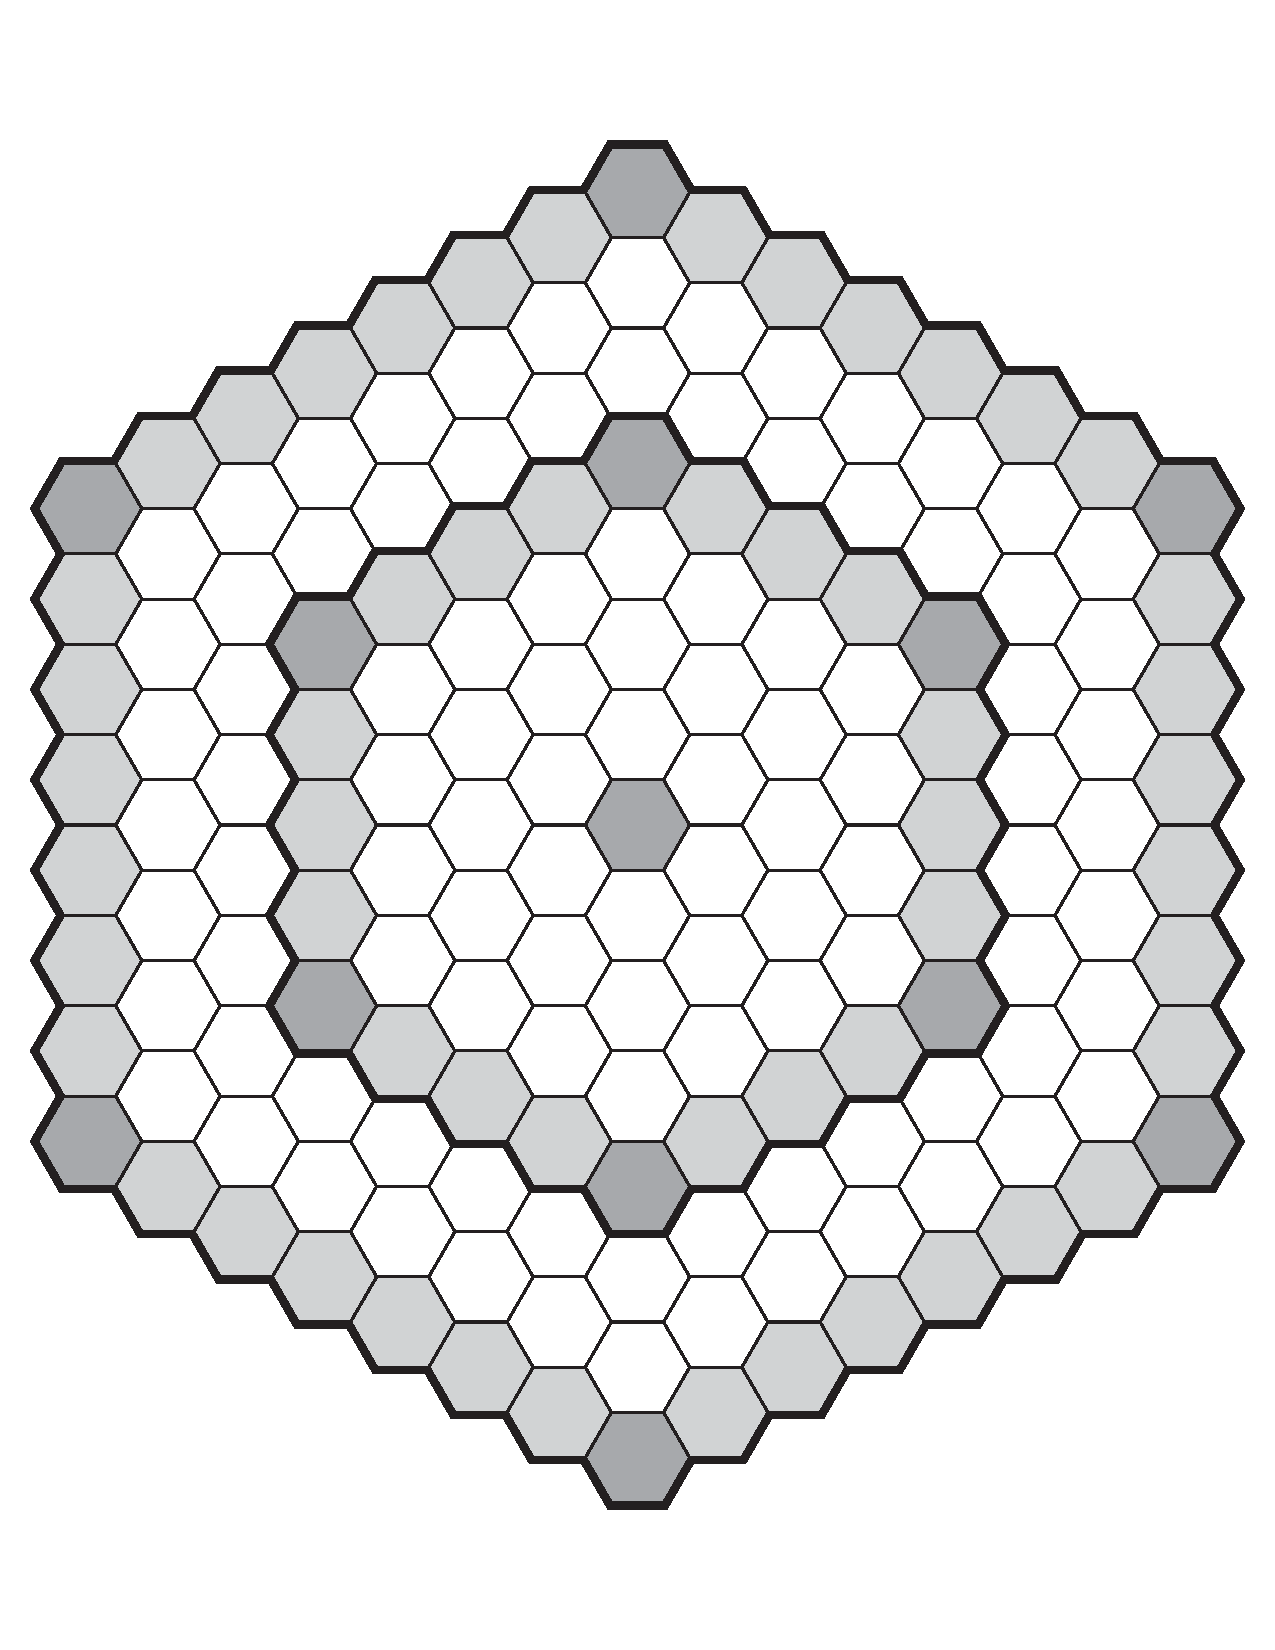
\includegraphics[width=200mm,clip=true,trim= 15pt 68pt 15pt 68pt]{boardsize8}
%width=\linewidth,
%\end{center}

%\centering
%\begin{HavannahBoard}[board size=4,coordinate style=classical,hex height=2.4cm]
%\end{HavannahBoard}

%\begin{HavannahBoard}[board size=5,coordinate style=classical,hex height=2cm]
%\end{HavannahBoard}

%\begin{HavannahBoard}[board size=6,coordinate style=classical,hex height=1.5cm]
%\end{HavannahBoard}

%\begin{HavannahBoard}[board size=7,coordinate style=classical,hex height=1.2cm]
%\end{HavannahBoard}

%\begin{HavannahBoard}[board size=8,coordinate style=classical,hex height=1cm]
%\end{HavannahBoard}




  % References - with commands to modify size and spacing
  \phantomsection
  \addcontentsline{toc}{chapter}{References}
  \small
  \renewcommand{\baselinestretch}{0.25}
  \bibliography{thesis}

\end{document}

